\chapter{Computational study}
\label{chap:computational_study}
This chapter will give the most insights into the functionality and efficiency of the usage of the presented binary classifier in
\gls{3L-CVRP} algorithms. This chapter will begin with the selection of two published \gls{3L-CVRP} datasets.
Afterwards the results from the model training are presented, which
is divided in three main parts, firstly the results of the retrieval of the data, secondly the feature selection, and finally presenting
different strategies for comparing different models and selecting the best best fit performance wise.
Afterwards a parameter study is conducted for the \gls{ILS}, starting with the \textit{NoClassifier} variant determining
the best configurations for the base parameters, followed by a variant specific parameter study.
This chapter closes with a computational study of all four variants, comparing the variants with tuned parameters.
These insights are summarized in the concluding chapter.

\section{Comparison of Available Datasets}
\label{sec:dataset_comparison}

The \gls{3L-CVRP} is a well-studied problem and several datasets were published in the past, considering
different constraints and characteristics. A selection of these datasets will be compared and evaluated
in this section. The goal is to identify suitable datasets for training a general \gls{CLP} classifier that can predict
the loading feasibility of single tours from different datasets. Therefore, the dataset needs
heterogeneous characterists to represent numerous possible use-cases
as shown in Section~\ref{sec:motivation_feasibility_prediction}. Five published
\cgls{3L-CVRP} datasets are presented with respect to their overall characteristics.
Each dataset gets an unique identfier to simplify the comparison and is shown in parenthesis
after the following individual introduction. The first \cgls{3L-CVRP} dataset was published by \citeauthor{gendreau_tabu_2006} in
\citeyear{gendreau_tabu_2006} and delivered the first \cgls{3L-CVRP} instances containing huge and heavy items (\gendreauDataSet).\footcite[cf.][]{gendreau_tabu_2006}
The second dataset was published by \citeauthor{moura_integrated_2009} in \citeyear{moura_integrated_2009},
and combines the \gls{VRP} from \citeauthor{solomon_algorithms_1987} and the \gls{CLP} instances from
\citeauthor{bischoff_issues_1995} defining the \gls{3L-VRPTW} considering
many items of small size and weight (\mouraDataSet).\footcites[cf.][]{solomon_algorithms_1987,bischoff_issues_1995}[][]{moura_integrated_2009}
The first dataset containing real-life data was published by \citeauthor{ceschia_local_2013} in \citeyear{ceschia_local_2013}
and contains the instances with the most items (\ceschiaDataSet).\footcite[cf.][]{ceschia_local_2013}
Krebs published two different datasets in
\citeyear{krebs_advanced_2021} with a focus on more realistic constraints. The first one contains a set
of realistic constraints and offers a wide range of instance sizes (\krebsADataSet).\footcite[cf.][]{krebs_advanced_2021}
The second one focuses on semi-trailer trucks and special requirements for axle weights (\krebsBDataSet).\footcite[cf.][]{krebs_axle_2021}
The characteristics of the datasets are summarized in the following Table~\ref{tab:dataset_comparison},
where the brackets [\,] indicate a range of possible values. All values considering mass and volume are
\textit{relative} to the respective vehicle weight and volume limit to be comparable. A \textit{item type} is
defined by its geometrical dimensions, the weight, and possible stability characteristics, such as fragility or \gls{LBS}.
When the number of item types is smaller than the number of items equal item types occur multiple times. The types column
depict the number of different item types per instance. Additionaly
most features of the dataset are compared with \textit{aggregated}  values, referring to the aggregrated characteristics
of all items requested by one customer, so the aggregated mass, volume and items shows the average value requested by an
customer of this dataset.

\newcolumntype{C}[1]{>{\centering\arraybackslash}p{#1}}
\newcolumntype{L}[1]{>{\raggedright\arraybackslash}p{#1}} % left-aligned
\begin{table}[ht]
    \centering
    \small
    \renewcommand{\arraystretch}{1.1}   % a touch more row height
    \begin{tabular}{@{}lccccc@{}}
        \toprule
        \textbf{Dataset} & \textbf{Instances} & \textbf{Customers} & \textbf{Agg. Mass}\footnote{Average is based on all customers of the instances.} & \textbf{Agg. Vol.} \footnotemark[\value{footnote}]       & \textbf{Agg. Items}\footnotemark[\value{footnote}] \\
        \midrule
        \gendreauDataSet & 27                 & [15, 100]          & 0.137                                                                            & 0.127                                                    & 2.00                                               \\
        \mouraDataSet    & 46                 & 25                 & 0.077                                                                            & 0.176                                                    & 52.0                                               \\
        \ceschiaDataSet  & 13                 & [11, 129]          & 0.063                                                                            & 0.160                                                    & 18.1                                               \\
        \krebsADataSet   & 600                & [20, 100]          & 0.098                                                                            & 0.100                                                    & 4.41                                               \\
        \krebsBDataSet   & 80                 & [30, 120]          & 0.036                                                                            & 0.052                                                    & 4.00                                               \\
        \toprule
        \textbf{Dataset} & \textbf{Items}     & \textbf{Types}     & \textbf{\text{Routes}}\footnote{Average is based on the instances.}              & \textbf{\text{Route Len}}\footnotemark[\value{footnote}] & \textbf{Fragility}\footnotemark[\value{footnote}]  \\
        \midrule
        \gendreauDataSet & [26, 199]          & [26, 199]          & 6.13                                                                             & 6.22                                                     & 0.25                                               \\
        \mouraDataSet    & 1050, 1550         & 5                  & 4.40                                                                             & 6.72                                                     & 0.29                                               \\
        \ceschiaDataSet  & [254, 8060]        & [9, 97]            & 10.2                                                                             & 5.81                                                     & 0.10                                               \\
        \krebsADataSet   & 200, 400           & 3, 10, 100         & 6.77                                                                             & 13.6                                                     & 0.24                                               \\
        \krebsBDataSet   & 200, 400           & 10, 100            & 3.87                                                                             & 22.1                                                     & 0.10                                               \\
        \bottomrule
    \end{tabular}
    \caption[Numerical comparison of different 3L--CVRP Datasets.]{Numeric comparisons between five avalaible datasets.}
    \label{tab:dataset_comparison}
\end{table}

The columns routes, route length and fragility show the average over all instances.
Routes define the \gls{LB} for the needed vehicles $K$ and route length the average number of customers per route based
on the relative volume and mass. The averages are displayed to become a better understanding of the
statistics of each dataset, rather than looking at extreme values.
The most important consideration, when selecting a suitable dataset for the training of a classifier,
is how representative single tours from one dataset are for all other datasets. Therefore, the numeric characteristics
should not contain outliers. It is apparent, that the \gendreauDataSetText dataset has the least items per customer
with huge relative volume and weight, which leads with an average route length of 6.22 customers to very few items
considered per route in comparison to the other datasets. This makes it easier to compute the feasibility of the loading
as the combinations of placing patterns is limited. The \mouraDataSetText dataset has the most items per average per customer consisting
of only 5 item types. The \ceschiaDataSetText dataset contains the fewest instances, but with the most maximum items of 8060,
which lead to many routes on average. The two datasets from Krebs, have similar
boundaries and values, but \krebsBDataSetText has routes with twice as many customers as \krebsADataSetText on average due
to the smaller average aggregated mass and volume. Both \krebsADataSetText and \gendreauDataSetText
show a good variety of the features, without including too many items per route in comparison to the other datasets.
However, as the average route length from \krebsADataSetText is twice as long and the number of items per customer contain twicw as many,
one route contain per average four times more items leading to a higher complexity for solving the \gls{CLP}.
The following Table~\ref{tab:constraint_matrix} provides an overview of the constraints considered
in each dataset showcasing the realistic profile. The constraints are categorized in the five loading constraint groups introduced
in Section~\ref{sec:clp_definition}.
\clearpage

\begin{table}[ht]
    \centering
    \small
    \renewcommand{\arraystretch}{1.2}
    \begin{tabular}{@{}L{1.8cm}L{3cm}C{1.6cm}C{1.6cm}C{1.6cm}C{1.6cm}C{1.6cm}@{}}
        \toprule
        \textbf{Category}          & \textbf{Constraint} &                        &                     & \textbf{Dataset}      &                      &                      \\
                                   &                     & Gendreau\newline(2006) & Moura\newline(2009) & Ceschia\newline(2013) & Krebs\newline(2021a) & Krebs\newline(2021b) \\
        \midrule
        \multirow{3}{*}{Container} & Load Capacity       & $\bullet$              & $\bullet$           & $\bullet$             & $\bullet$            & $\bullet$            \\
                                   & Load Balance        &                        &                     &                       & $\bullet$            &                      \\
                                   & Axle Weights        &                        &                     &                       & $\bullet$            & $\bullet$            \\\midrule
        \multirow{3}{*}{Item}      & z-Rotation          & $\bullet$              & $\bullet$           & $\bullet$             & $\bullet$            & $\bullet$            \\
                                   & Fragility           & $\bullet$              &                     & $\bullet$             & $\bullet$            & $\bullet$            \\
                                   & LBS                 &                        &                     & $\bullet$             & $\bullet$            &                      \\\midrule
        \multirow{1}{*}{Cargo}     & Complete Shipm.     & $\bullet$              & $\bullet$           &                       & $\bullet$            & $\bullet$            \\\midrule
        \multirow{6}{*}{Position}  & Geometry            & $\bullet$              & $\bullet$           & $\bullet$             & $\bullet$            & $\bullet$            \\
                                   & Orthogonality       & $\bullet$              & $\bullet$           & $\bullet$             & $\bullet$            & $\bullet$            \\
                                   & Reachability        &                        &                     & $\bullet$             & $\bullet$            &                      \\
                                   & Sequence            & $\bullet$              &                     &                       & $\bullet$            &                      \\
                                   & LIFO                & $\bullet$              & $\bullet$           & $\bullet$             & $\bullet$            & $\bullet$            \\
                                   & MLIFO               &                        &                     & $\bullet$             & $\bullet$            &                      \\\midrule
        \multirow{2}{*}{Load}      & Robust Stability    &                        &                     & $\bullet$             & $\bullet$            &                      \\
                                   & Support Area        & $\bullet$              & $\bullet$           &                       &                      & $\bullet$            \\

        \bottomrule
    \end{tabular}
    \caption[Overview of CLP constraints in selected 3L--CVRP datasets.]{Matrix overview of constraints covered in selected datasets. A bullet ($\bullet$) indicates that the constraint is considered.}
    \label{tab:constraint_matrix}
\end{table}

This comparison shows that all datasets include similar types of constraints, but the level
of complexity varies. \krebsADataSetText and \ceschiaDataSetText stand out by incorporating
more advanced constraints such as robust stability, reachability, and \gls{LBS}, in comparison to
basic ones like support area, \gls{LIFO} and fragility. To further investigate the differences
between the datasets, Figure~\ref{fig:dataset_comparison} visualizes the aggregated relative mass and
volume of all items requested by individual customers.
Additionally, the size of each scatter point indicates the total number of items requested.
For example, the \mouraDataSetText dataset includes 46
instances with 25 customers each, resulting in $25 \cdot 46 = 1150$ dots in the plot.

\begin{figure}[ht]
    \centering
    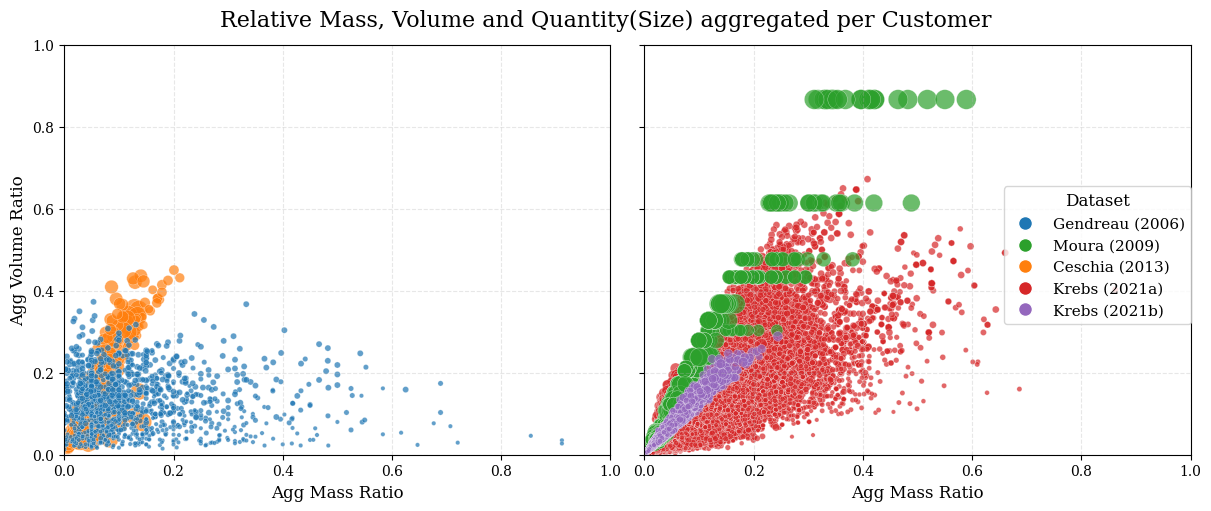
\includegraphics[width=0.85\textwidth]{pictures/comparison_datasets_3lcvrp.png}
    \caption{Comparison aggregated customer demands of different 3L--CVRP/ 3L--VRPTW datasets.}
    \label{fig:dataset_comparison}
\end{figure}

The dispersion of the data points reflects the diversity of individual instances in terms of volume
and mass dependency. A more balanced profile suggests that some customers tend to order items that
are either mass- or volume-intensive, which supports training the model on more heterogeneous data.
Therefore, the dataset should cover a wide range of cases, varying in mass, volume, and item
quantity per customer. The widest spread is observed in \krebsADataSetText and \gendreauDataSetText serving
both as good dataset candidates for training a classifier. Both datasets are investigated further in
the next section.

\section{Analsis of datasets}
\label{sec:analysis_datasets}

The two datasets, \krebsADataSetText and \gendreauDataSet, have a good diverse profile for training
a binary classifier and to be further analyzed.
As shown in Section~\ref{sec:literature_overview} several publications solved the \gendreauDataSetText dataset
with various heuristics and even exact approaches, whereas only one heuristic solution approach exists for the instances of \krebsADataSet.
Both datasets are further analysed in this section to understand dataset specific properties.

\subsubsection{\krebsADataSetText}

The dataset contains 600 instances with 18 instance types derived from the combinations
of number of customers, item types and items. The following Figure~\ref{fig:krebs_dataset_analysis_detailes} plots
the relative mass and volume of all items requested by individual customers for each of the instances. Every color
represents one instance type and the plots are divided by the number of respective customers in three groups, presenting
6 combinations each. There are three levels for the different item types per [3,10,100] and two levels for the total
number of items, 200 and 400, per instance.
\begin{figure}[ht]
    \centering
    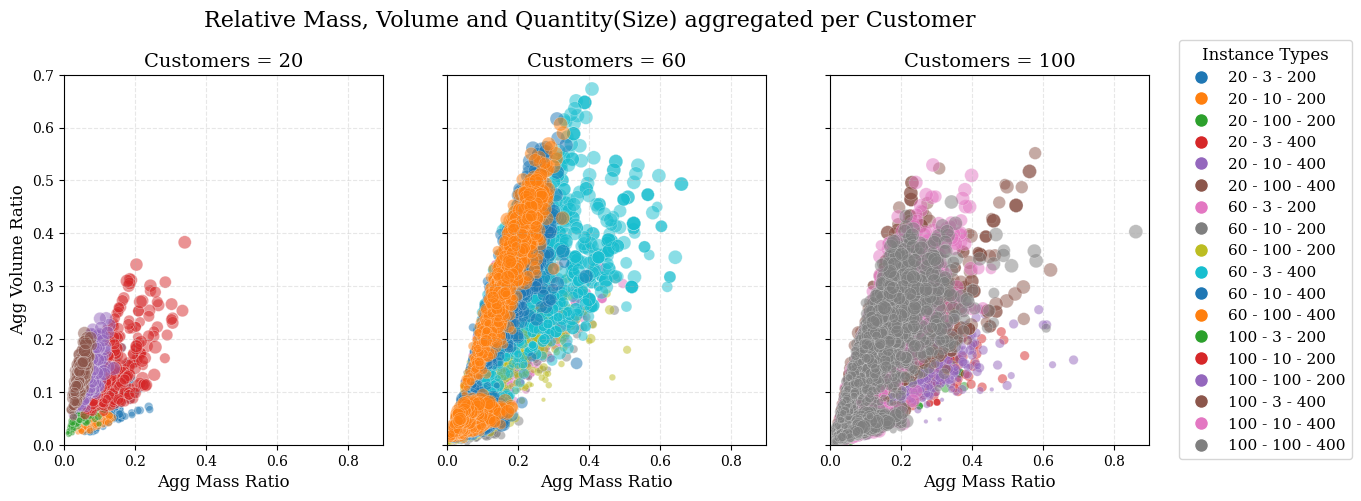
\includegraphics[width=0.85\textwidth]{pictures/krebs_instances_detailed.png}
    \caption[Visualization of different instances of \textcite{krebs_advanced_2021} dataset.]{Visualization of different instances of \krebsADataSetText dataset.
        The instances are named by the number of customers, item types and items.}
    \label{fig:krebs_dataset_analysis_detailes}
\end{figure}%
Several insights can be obtained from the analysis of this plot. Firstly, the aggregated relative
volume and mass per customer is significantly lower for the group with 20 customers than for the groups with 60 or 100 customers.
Secondly, the distribution differs from each instance type, ranging from quite linear distributions in a narrow
interval (e.g. instance 60-100-400) to quite broad distributions (e.g. instance 100-100-400). These two observations need to be considered,
when selecting instances to generate the training data for the classifier to avoid a homogenous training sets.
The instance set should be drawn from every group equally and different distributions need to be considered per group,
that the average numeric route structure differs.

\subsubsection{\gendreauDataSetText}

This dataset consists of 27 instances, where the dispersion of the aggregated mass per customer is reaching very high values, up to
0.91, but has modest volume levels, with a maximum of 0.4 approximately, as could be seen in Figure~\ref{fig:dataset_comparison}. The
following Figure~\ref{fig:aggregated_gendreau_plots} show this dispersion per instance revealing an important insight about the dataset.
As the relative volume is quite constant for all instances, the relative mass differs between the instances.
\begin{figure}[ht]
    \centering
    \begin{tikzpicture}[scale=0.9, transform shape,node distance=0mm and 0mm]
        \node[anchor=south, inner sep=0] (A) at (0,0)
        {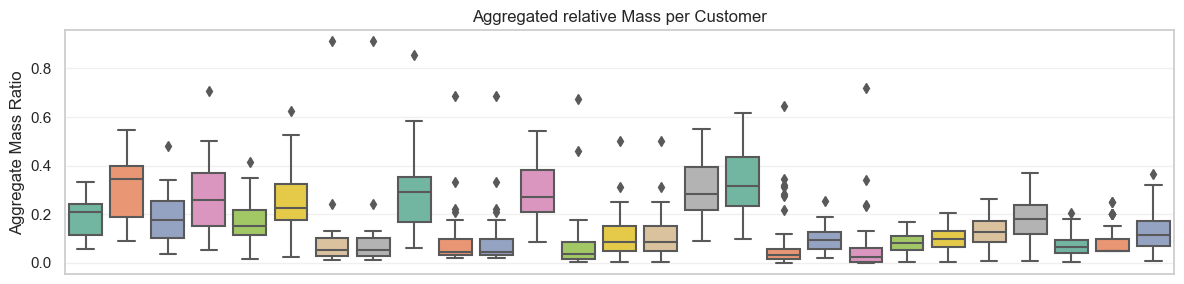
\includegraphics[width=0.95\textwidth]{pictures/AggMassCustGendreau.png}};
        \node[anchor=north, below=of A,inner sep=0] (B)
        {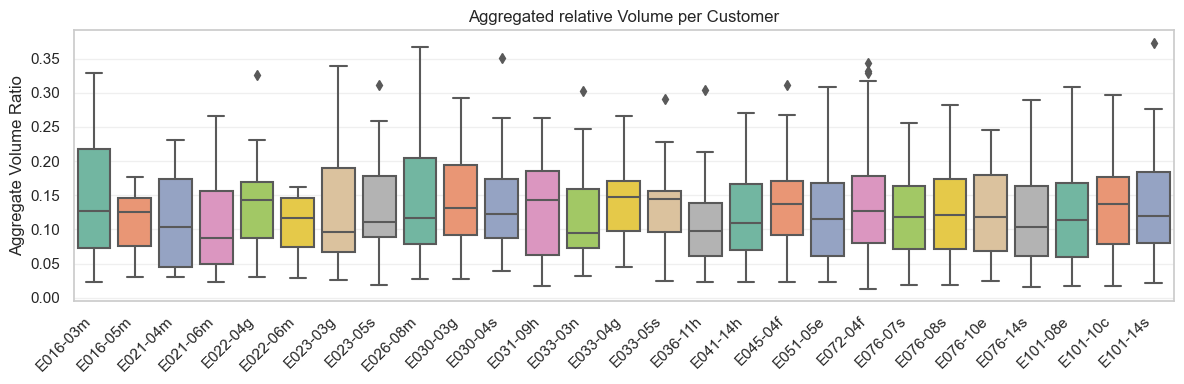
\includegraphics[width=0.96\textwidth]{pictures/AggVolCustGendreau.png}};
    \end{tikzpicture}
    \caption{Aggregated relative mass and volume per customer distributed for each instance of the \gendreauDataSetText dataset.}
    \label{fig:aggregated_gendreau_plots}
\end{figure}
As it was analyzed from \cite{tamke_branch-and-cut_2024}
the complexity to solve the instances is far greater, when the items are more lightweight and the volume is the limiting factor
for packing items in the container. Furthermore, the authors distinguished the instances in a
group of heavy items ($\mathcal{H}$) and a group of lighweight items ($\mathcal{L}$) by the average weight utilization $\overline{\omega}$
of the final routes obtained.\footcite[cf.][pp. 23-25]{tamke_branch-and-cut_2024}
As this classification is based on the optimal solutions, another approach will be followed ifn this thesis to distinguish both
\krebsADataSetText and \gendreauDataSetText in heavy (H) and lightweight (L) items. An instance is accounted as heavyweigt, if
the average weight aggregated per customer is above the average over all instances. This definition has the advantage, that also instances absent
of optimal / good solutions can be labeled. The obtained results for the \gendreauDataSetText and \krebsADataSetText instances will be
differentiated in those two groups to investigate the effect of the average weight per customer on the solution quality and process.

\parbreak

As the construction of train datasets with the \krebsADataSetText dataset is much more computationally challenging than for \gendreauDataSet,
the following sections will focus only on the latter and the Section~\ref{sec:application_krebs} on solving instances from \krebsADataSet.
In the following section the results from training the binary classifier
are presented with diffferent datasets.

\section{Results Model Training}
\label{sec:ResultsTraining}
In this section the results from the feature dataset selection are discussed. The single best features
with individual scores are shown in the Appendix~\ref{app:feature_selection}. For each model variant (see Section~\ref{sec:modelselection})
the most suiting dataset is selected from both, the Random Retrieval and Save Strategy datasets. These selected
models will then be used in the further steps of the computational study to compare the \gls{ILS} algorithm
with and without the boost of the classifier. Additionally, the Section~\ref{app:sec:krebs_computationally_challenges} in the appendix
dives deeper in the challenges for creating a suiting training dataset from the \krebsADataSetText instances and the computational
challenges.

\subsubsection{Random Retrieval Strategy}
The following random datasets were created with the Algorithm~\ref{fig:flowchart_randomRouteGeneration}. All instances
from \gendreauDataSetText were considered. It must be noted, that the parameter for attempts limit $\beta$ did not have a huge influence on
the number of routes and the structure of the dataset. Therefore only the datasets with $\beta = 30$ have been preselected.
The values in the balance column stand for the share of positive and negative labels in the sample population. The relative volume
and mass refer to the average value for all routes in the respective dataset. The names for the random datasets are constructed from
the parameters as follows: RD-$\alpha$-$\beta$-$\gamma$-$10\delta$.

\begin{table}[ht]
    \centering
    \small
    \begin{tabular}{@{}L{0.20\textwidth}P{0.04\textwidth}P{0.04\textwidth}P{0.05\textwidth}P{0.10\textwidth}P{0.12\textwidth}P{0.12\textwidth}P{0.12\textwidth}@{}}
        \toprule
        Name          & $\alpha$           & $\gamma$            & $\delta$ & Routes & Balance   & Rel. Vol & Rel. Mass \\
        \midrule
        RD-2-30-20-6  & \multirow{3}{*}{2} & \multirow{3}{*}{20} & 0.6      & 36779  & 34.4/65.6 & 0.66     & 0.55      \\
        RD-2-30-20-8  &                    &                     & 0.8      & 40724  & 29.0/71.0 & 0.69     & 0.59      \\
        RD-2-30-20-10 &                    &                     & 1        & 47350  & 24.3/75.7 & 0.75     & 0.65      \\
        \midrule
        RD-2-30-30-6  & \multirow{3}{*}{2} & \multirow{3}{*}{30} & 0.6      & 56644  & 33.6/66.4 & 0.66     & 0.55      \\
        RD-2-30-30-8  &                    &                     & 0.8      & 63011  & 28.2/71.8 & 0.69     & 0.59      \\
        RD-2-30-30-10 &                    &                     & 1        & 72408  & 24.2/75.8 & 0.75     & 0.6       \\
        \midrule
        RD-3-30-20-6  & \multirow{3}{*}{3} & \multirow{3}{*}{20} & 0.6      & 48987  & 35.4/64.6 & 0.65     & 0.54      \\
        RD-3-30-20-8  &                    &                     & 0.8      & 61376  & 28.8/71.2 & 0.69     & 0.59      \\
        RD-3-30-20-10 &                    &                     & 1        & 70843  & 24.5/75.5 & 0.74     & 0.64      \\
        \midrule
        RD-3-30-30-6  & \multirow{3}{*}{3} & \multirow{3}{*}{30} & 0.6      & 84751  & 33.8/66.2 & 0.66     & 0.55      \\
        RD-3-30-30-8  &                    &                     & 0.8      & 93942  & 28.6/71.4 & 0.69     & 0.59      \\
        RD-3-30-30-10 &                    &                     & 1        & 108597 & 24.0/76.0 & 0.75     & 0.65      \\
        \midrule
        RD-4-30-20-6  & \multirow{3}{*}{4} & \multirow{3}{*}{20} & 0.6      & 73549  & 34.4/65.6 & 0.66     & 0.55      \\
        RD-4-30-20-8  &                    &                     & 0.8      & 81607  & 28.9/71.1 & 0.69     & 0.59      \\
        RD-4-30-20-10 &                    &                     & 1        & 94666  & 24.2/75.8 & 0.75     & 0.65      \\
        \midrule
        RD-4-30-30-6  & \multirow{3}{*}{4} & \multirow{3}{*}{30} & 0.6      & 113241 & 33.7/66.3 & 0.66     & 0.55      \\
        RD-4-30-30-8  &                    &                     & 0.8      & 125181 & 28.4/71.6 & 0.69     & 0.59      \\
        RD-4-30-30-10 &                    &                     & 1        & 144311 & 24.1/75.9 & 0.75     & 0.65      \\
        \midrule
        RD-5-40-40-6  & \multirow{3}{*}{5} & \multirow{3}{*}{40} & 0.6      & 197525 & 32.0/68.0 & 0.67     & 0.56      \\
        RD-5-40-40-8  &                    &                     & 0.8      & 217085 & 27.3/72.7 & 0.70     & 0.60      \\
        RD-5-40-40-10 &                    &                     & 1        & 249762 & 23.1/76.9 & 0.76     & 0.66      \\
        \bottomrule
    \end{tabular}
    \caption{Created instances for different parameter combinations $(\alpha, \beta, \gamma, \delta)$ for \gendreauDataSetText dataset.}
    \label{tab:created_instances_xyz_gendreau}
\end{table}
The greatest impact on the route characteristics contained in the datasets has parameter $\delta$ as fewer and lighter packed routes
are created. The route characteristics of balance and relative volume and weight are nearly identical for each other tuple combination
of ($\alpha$,$\beta$,$\gamma$). This influence is visualized in the following Figure~\ref{fig:route-dists_randomdata}, where the distribution
of the route length of each $\delta$ variant is shown for an exemplary random dataset.

\begin{figure}[!ht]
    \centering
    \begin{subfigure}[t]{.33\textwidth}
        \centering
        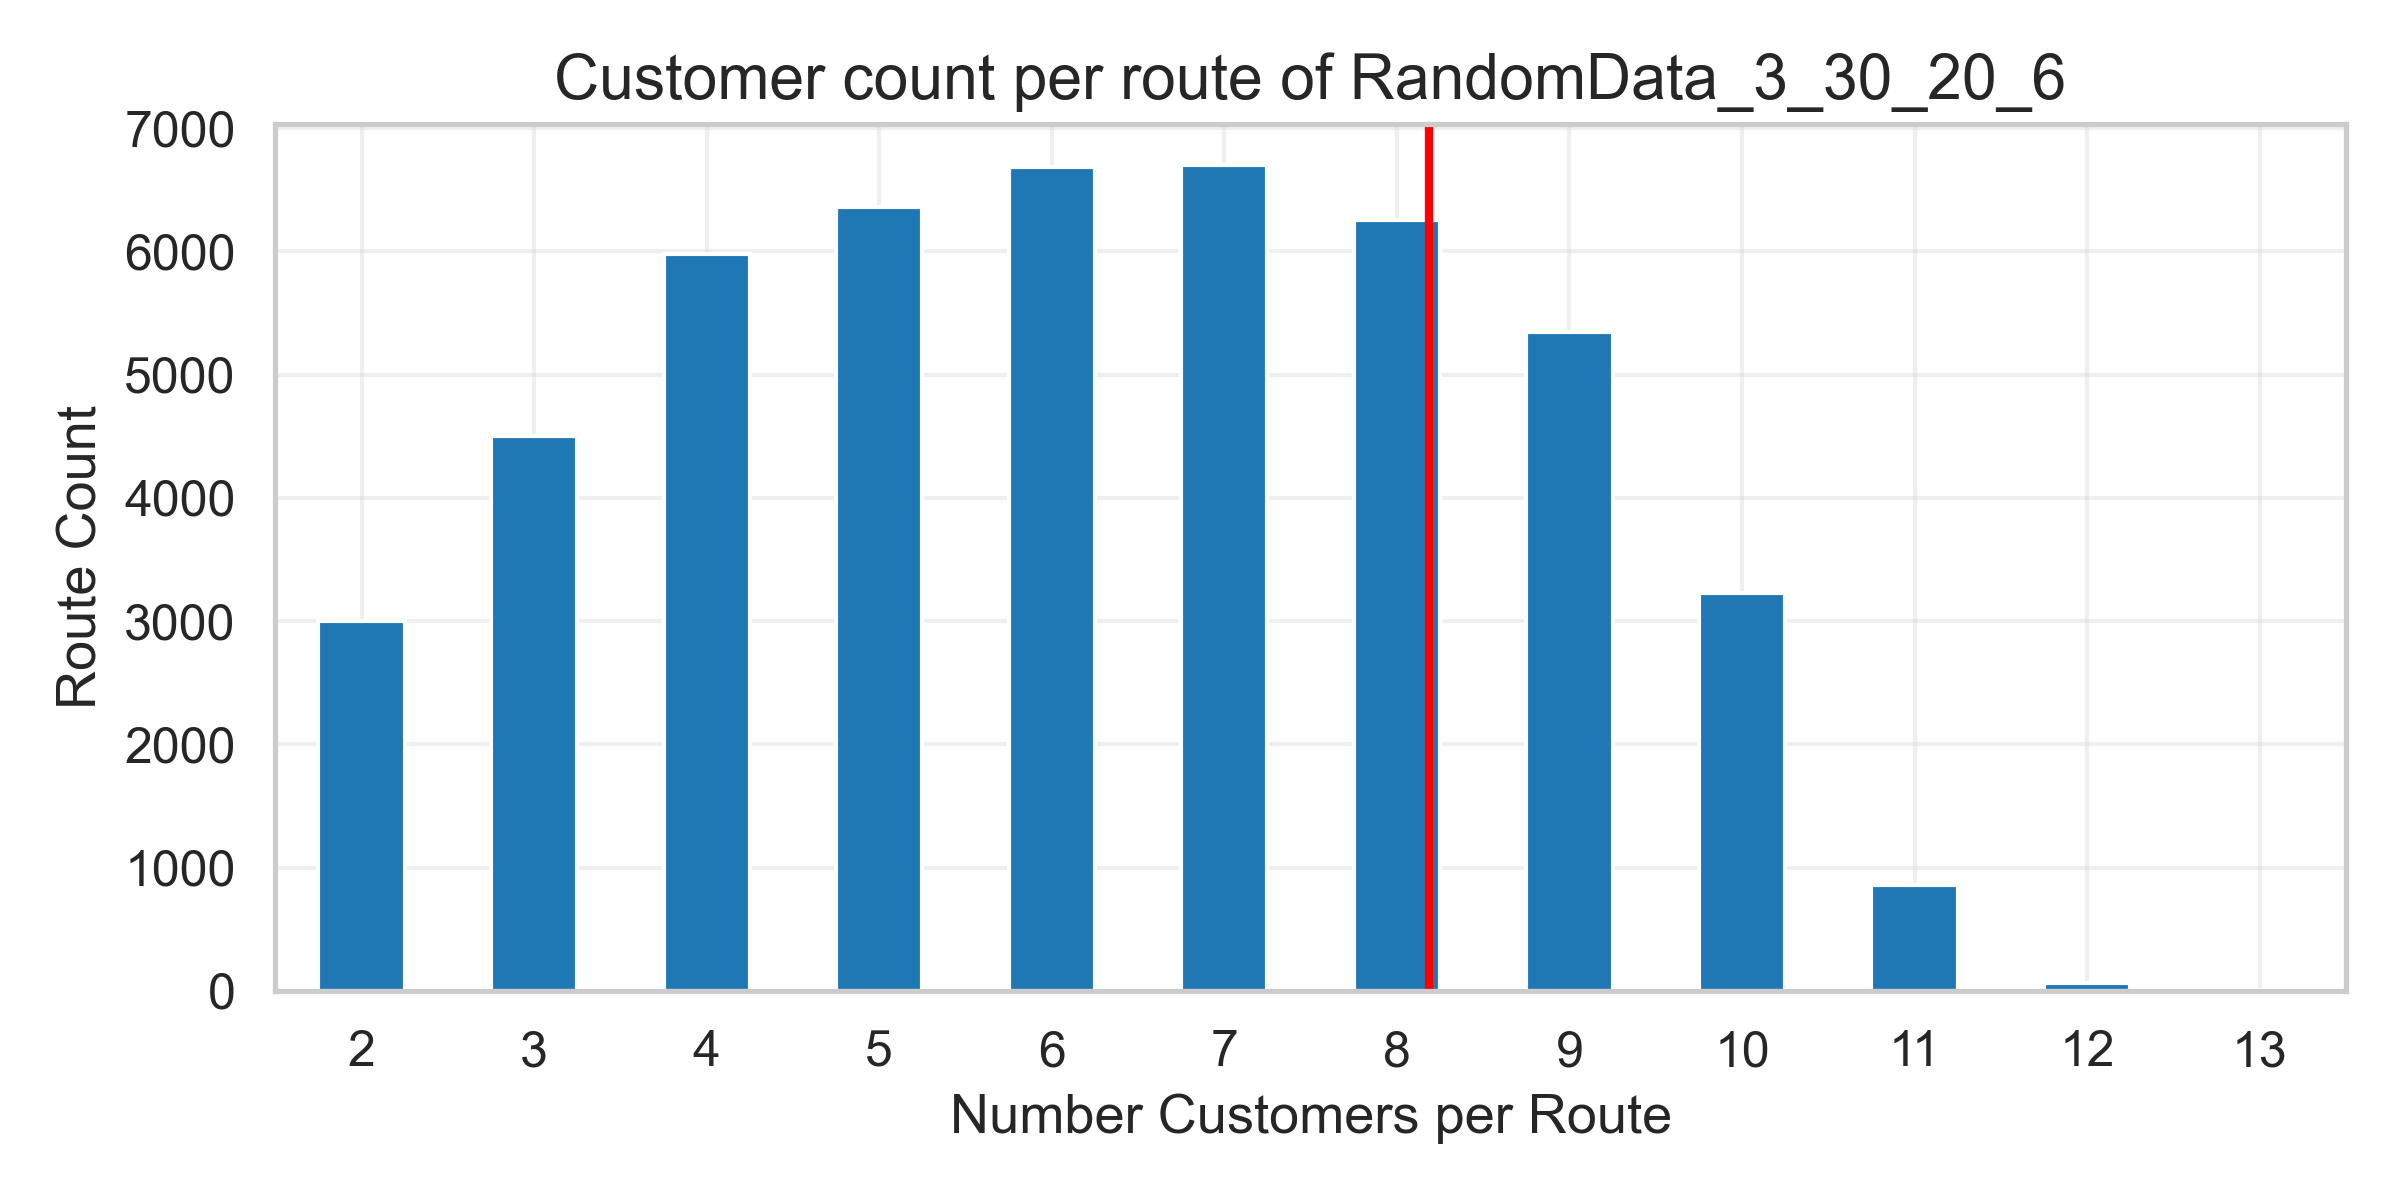
\includegraphics[width=\linewidth]{pictures/dataset_structure/no_cust_plot_RandomData_3_30_20_6.png}
        \caption{RD-3-30-20-6; \\Threshold $\delta$ = 0.6.}
        \label{fig:ds-a}
    \end{subfigure}%
    \begin{subfigure}[t]{.33\textwidth}
        \centering
        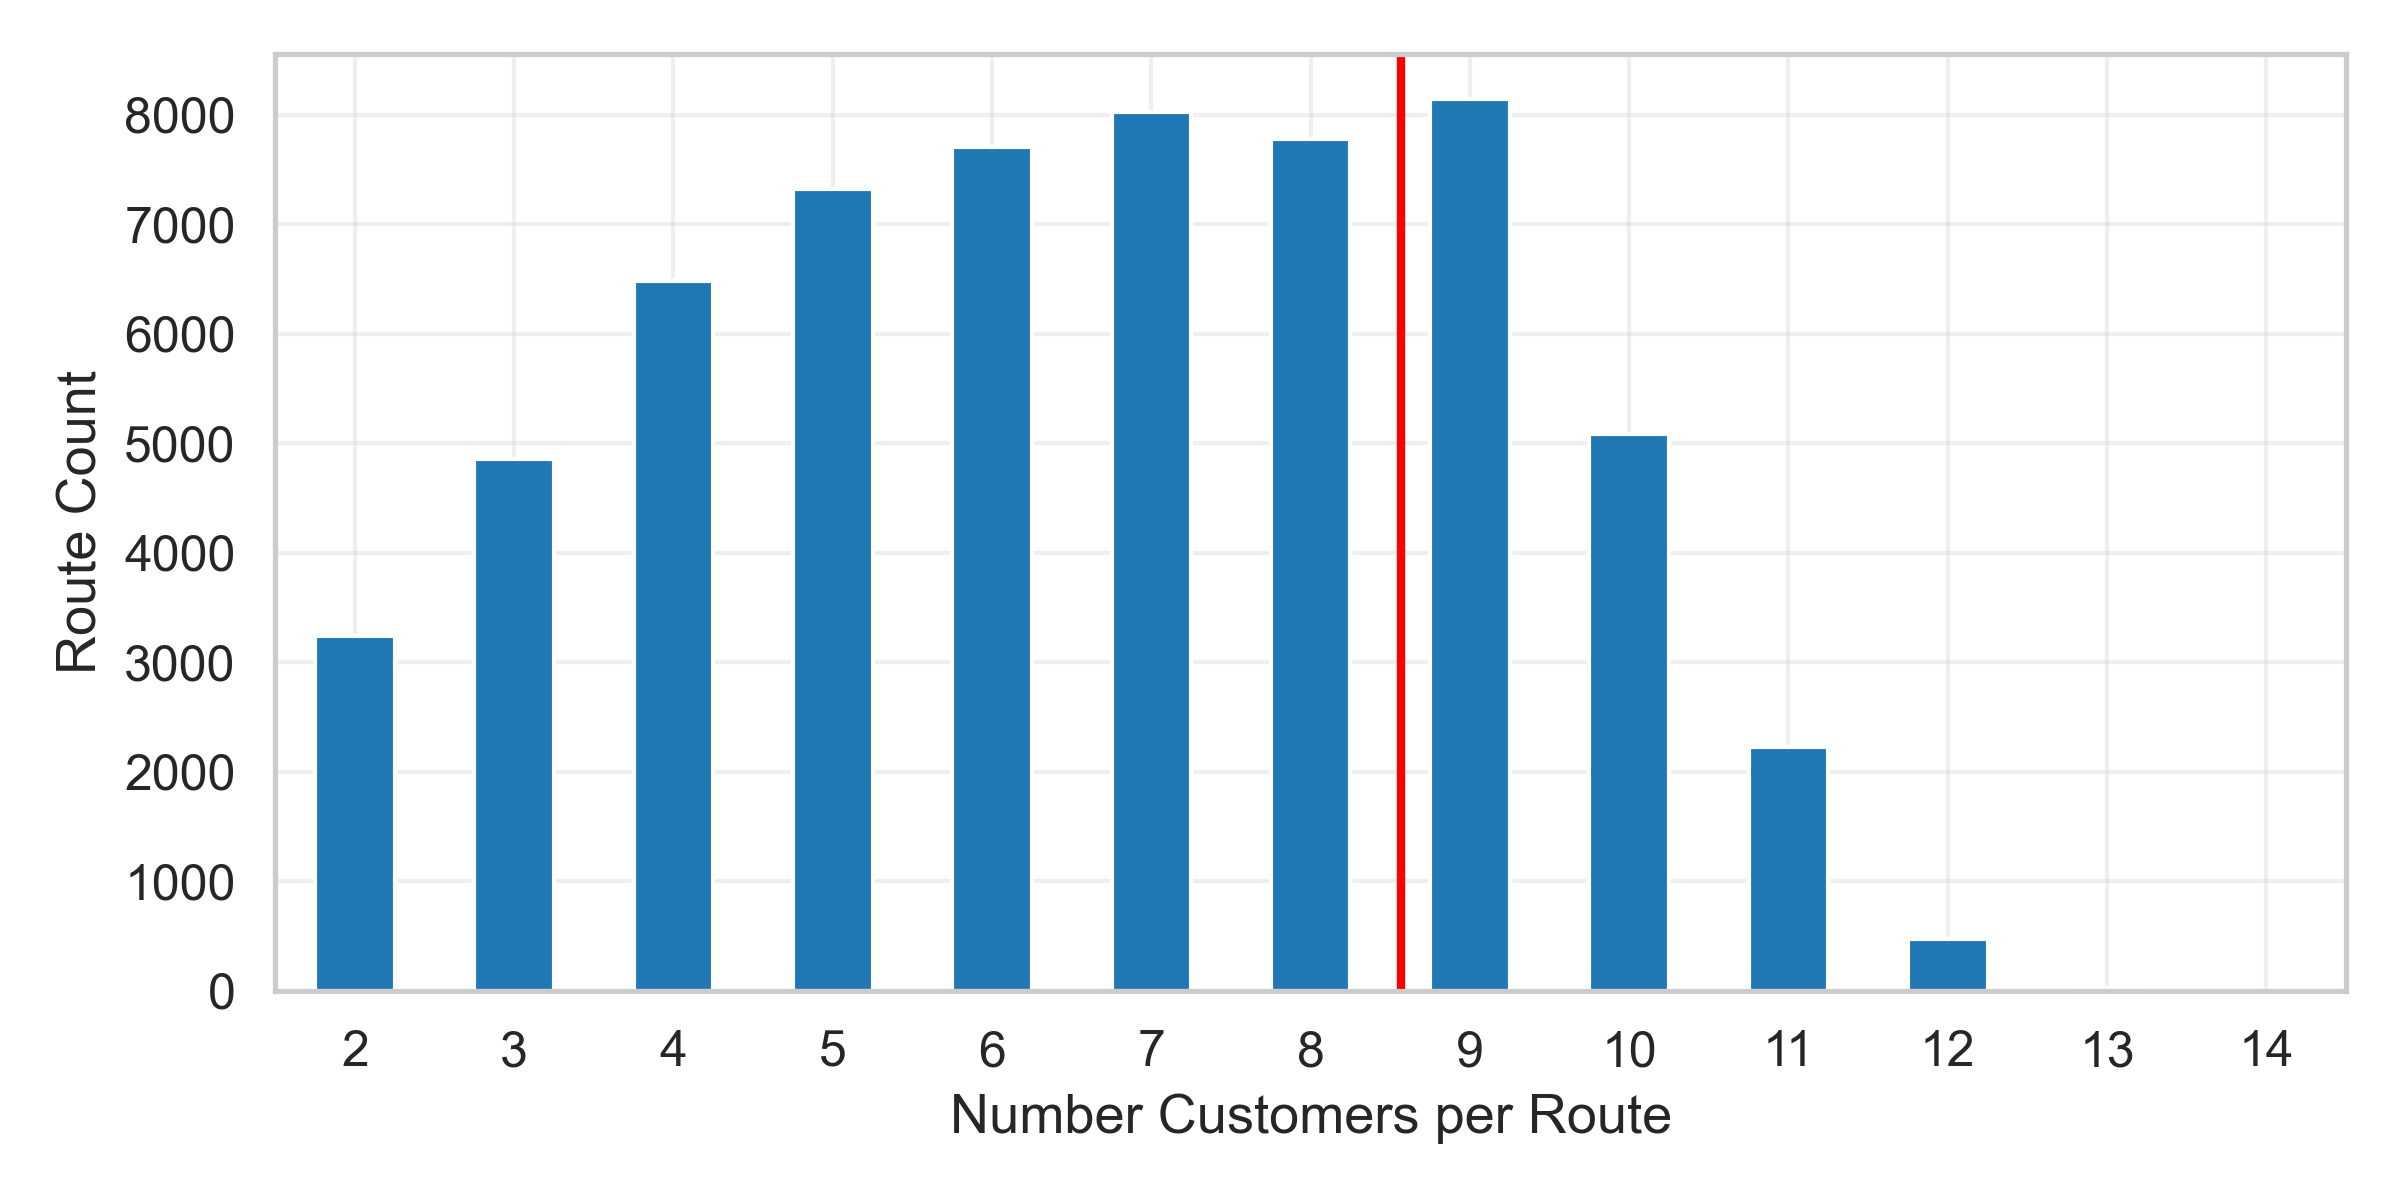
\includegraphics[width=\linewidth]{pictures/dataset_structure/no_cust_plot_RandomData_3_30_20_8.png}
        \caption{RD-3-30-20-8; \\Threshold $\delta$ = 0.8.}
        \label{fig:ds-b}
    \end{subfigure}
    \begin{subfigure}[t]{.33\textwidth}
        \centering
        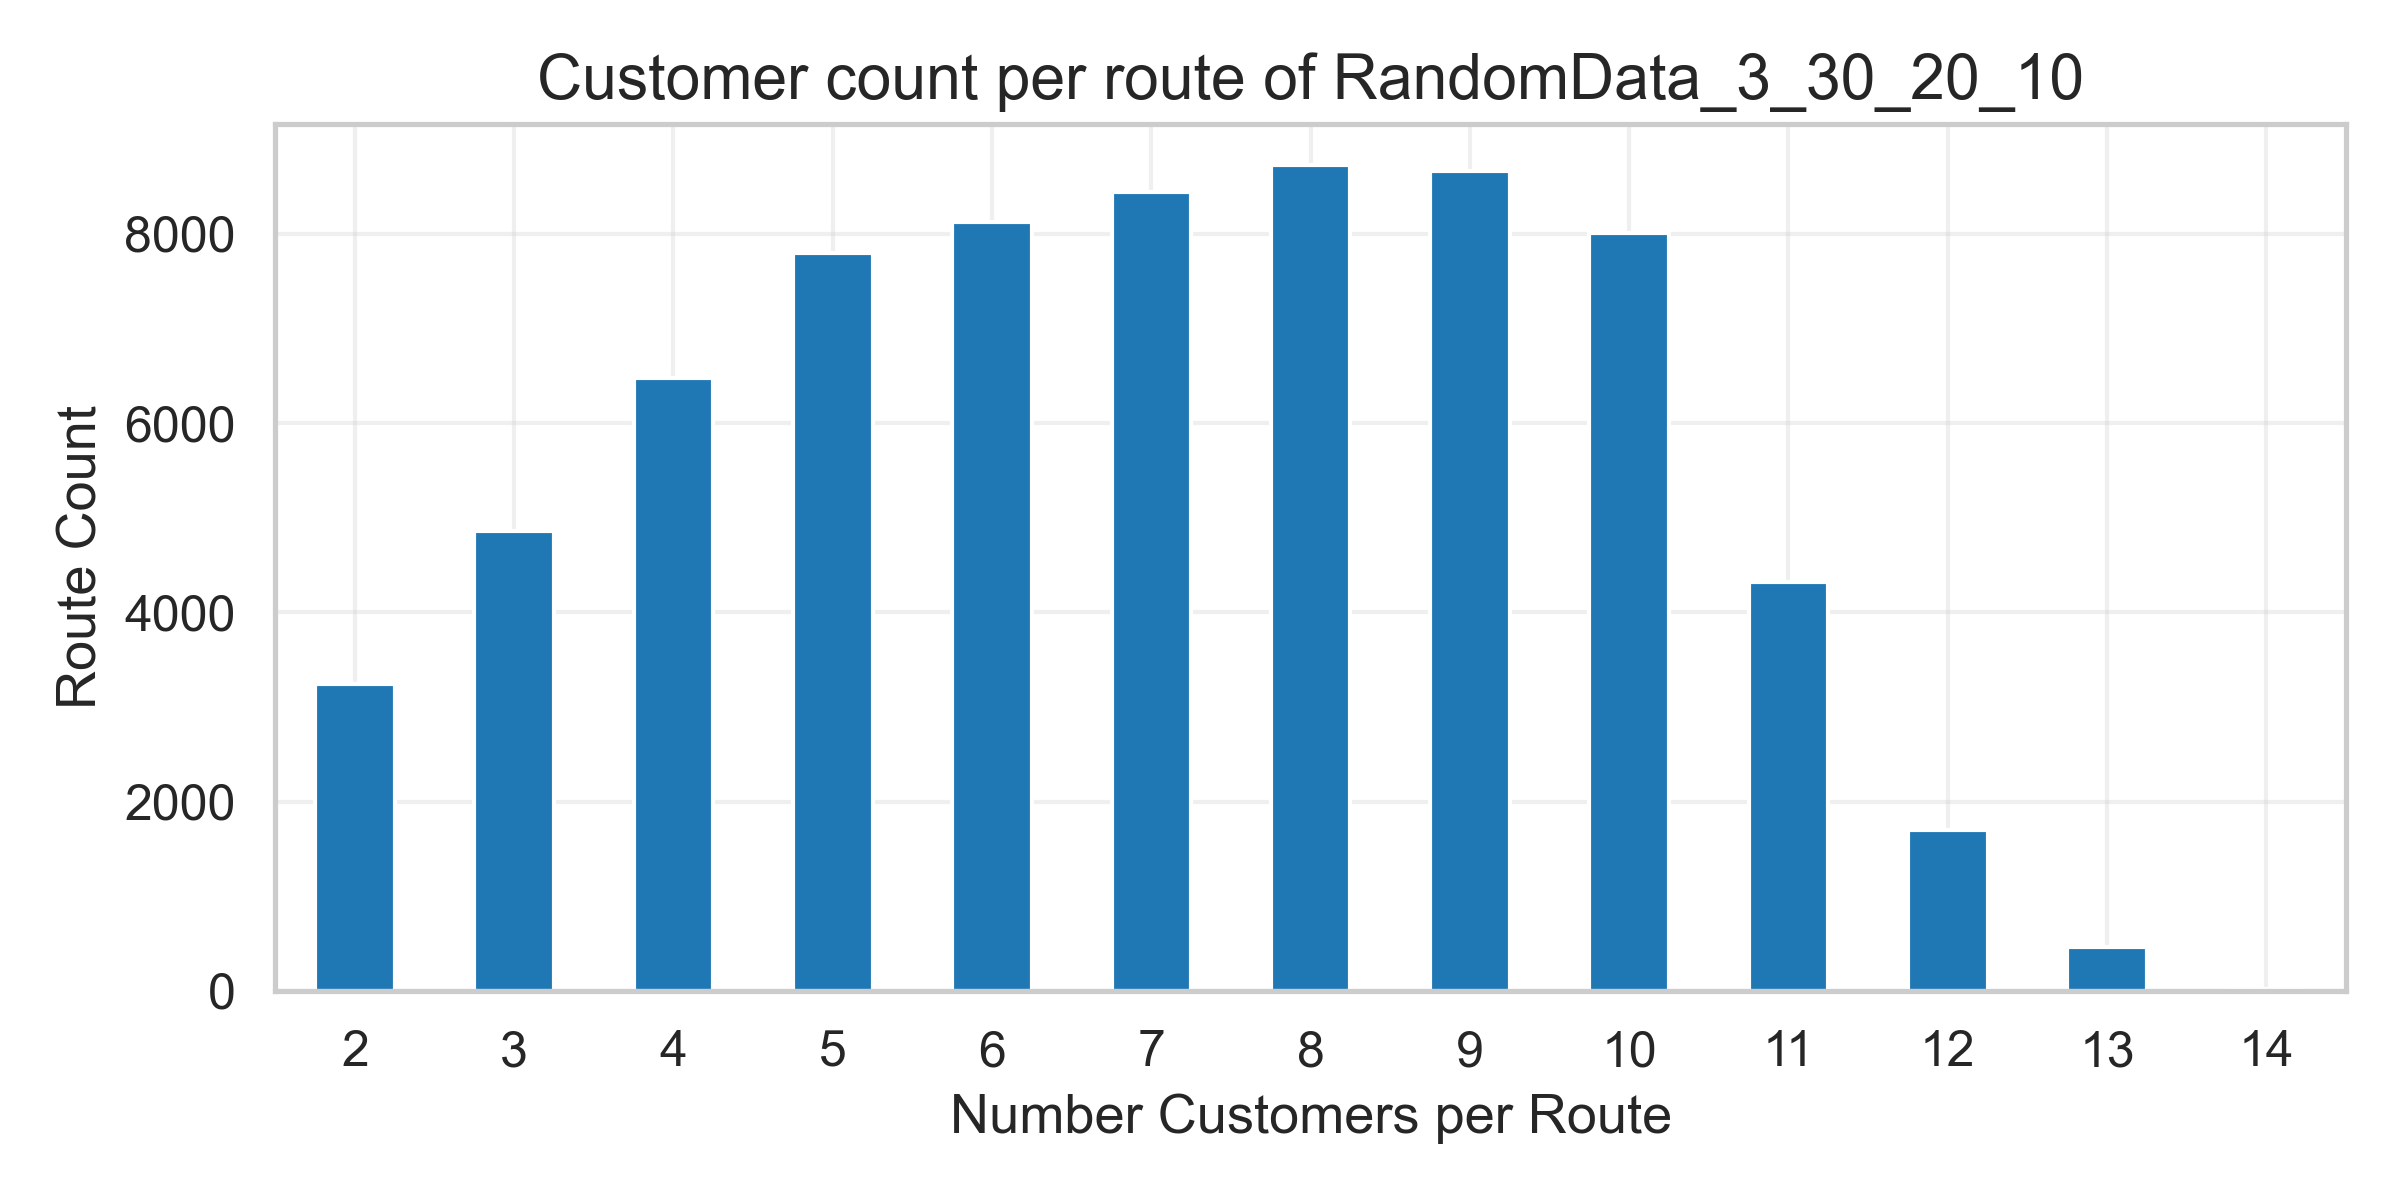
\includegraphics[width=\linewidth]{pictures/dataset_structure/no_cust_plot_RandomData_3_30_20_10.png}
        \caption{RD-3-30-20-10; \\ Threshold $\delta$ = 1.0.}
        \label{fig:ds-c}
    \end{subfigure}
    \caption[Distribution of route length for the random strategy with different thresholds.]{Distribution of route length the random strategy for with different thresholds.
        The red vertical line represents the average number of customers.}
    \label{fig:route-dists_randomdata}
\end{figure}

\FloatBarrier

\subsubsection{Save Retrieval Strategy}

By running the complete B\&C algorithm from \cite{tamke_branch-and-cut_2024}, two train datasets were generated,
one considering additionally the infeasible routes constructed from the \textit{NoSequence} sets and one only the sequences.
The prior dataset is labeled with WS (= with sets) (see Section~\ref{sec:DataRetrieval}). The length of the routes included in the
train dataset are dominated by routes consisting of two customers,
as in the beginning of the algorithm all customer combinations are checked to find infeasible customers tuple to
fasten the feasibility loading check in the algorithm afterwards, which is shown in Figure~\ref{fig:customer_count_bc}. \footcite[cf.][]{tamke_branch-and-cut_2024}
The results of the branch-and-cut algorithm are summarized in Table~\ref{tab:bc_results_gendreau} in the appendix.
\begin{wrapfigure}{l}{0.5\textwidth}
    \begin{center}
        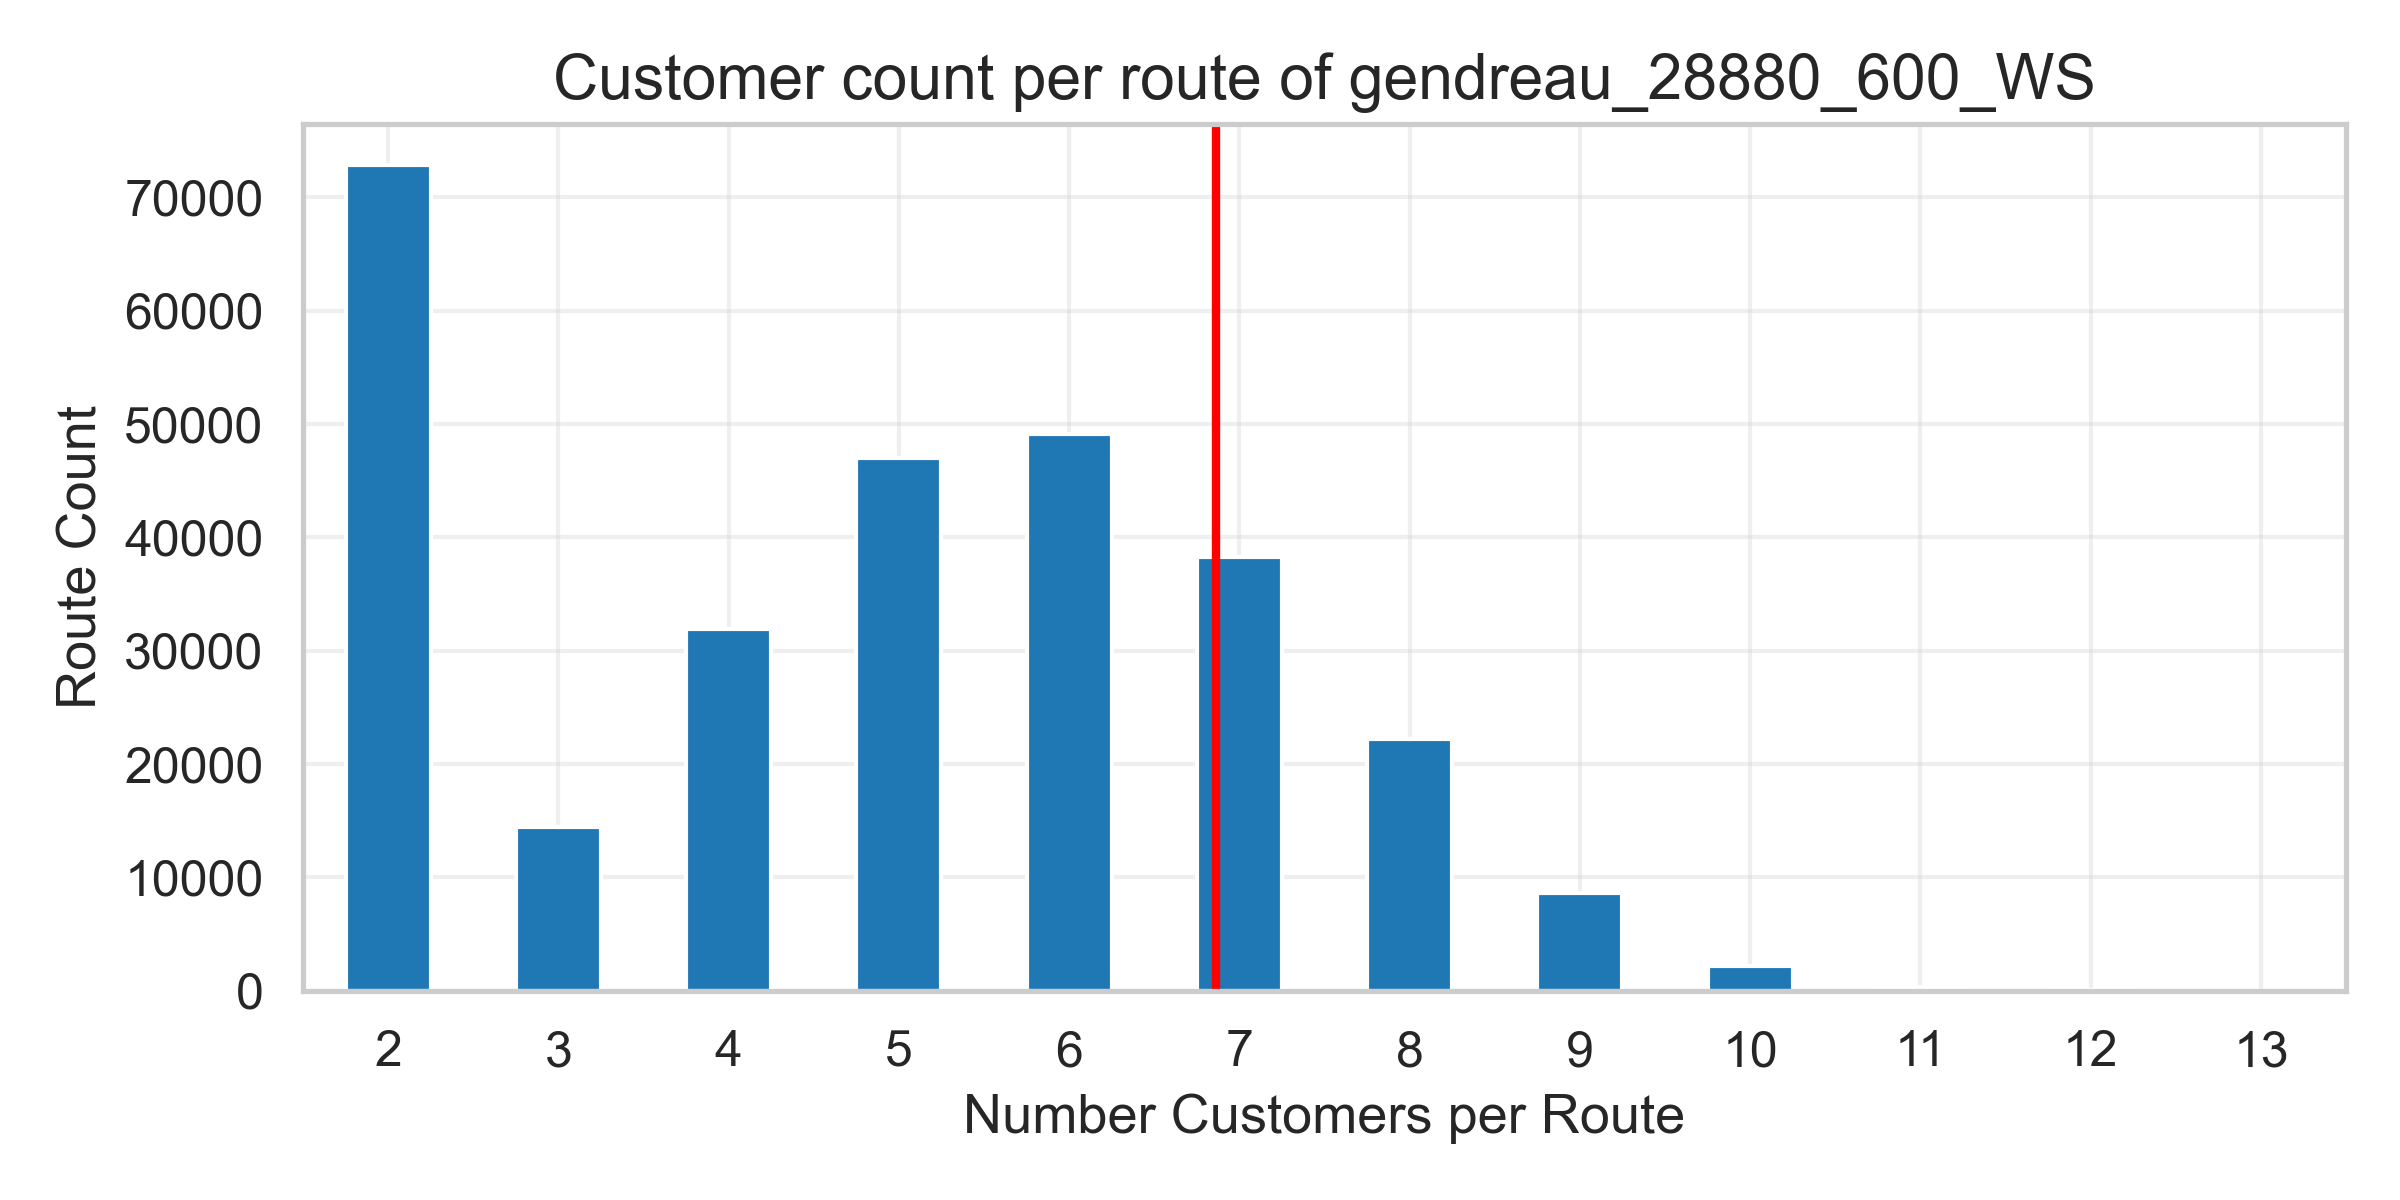
\includegraphics[width = .5\textwidth]{pictures/dataset_structure/no_cust_plot_gendreau_28880_600_WS.png}
        \caption{Customer count per route for dataset GD-Complete-WS.}
        \label{fig:customer_count_bc}
    \end{center}
\end{wrapfigure}
To reduce the number of routes with two customers, two alternative datasets are constructed for each base dataset (Complete) to test if the reduction
of number of routes with 2 customers, lead to better model performance results. Therefore it was tested
to shrink all feasible routes with 2 customers with a cosine similarity of $94\%$ (Shrinked) or alternatively drop
all feasible routes with 2 customers (Trimmed).
The resulting datasets have the following characterics, shown in Table~\ref{tab:saved_instances_gendreau}, and it is apparent, that the average relative volume
and mass are higher for the two modified datasets, as short routes were dropped. Additionally the balance between
feasible and infeasible is tilting to more to infeasible tours as only feasible routes with two customers were dropped.
Additonally the WS datasets contain more infeasible routes and are therefore more imbalanced. The use case of the trimmed dataset is limited,
as no feasible short tours are included. This distorts the application of the model classifier, since small tours are only labeled as infeasible.

\begin{table}[!h]
    \centering
    \small
    \begin{tabular}{l c c c c c c }
        \toprule
        Name           & Sets                 & Routes & Route Len = 2 & Balance   & Rel. Vol & Rel. Mass \\
        \midrule
        GD-Complete-WS & \multirow{3}{*}{Yes} & 286858 & 72832         & 37.6/62.4 & 0.62     & 0.46      \\
        GD-Trimmed-WS  &                      & 216260 & 2234          & 17.2/82.8 & 0.74     & 0.54      \\
        GD-Shrinked-WS &                      & 249564 & 35538         & 28.2/71.8 & 0.68     & 0.50      \\        \midrule
        GD-Complete    & \multirow{3}{*}{No}  & 220825 & 72832         & 48.8/51.2 & 0.55     & 0.43      \\
        GD-Trimmed     &                      & 150227 & 2234          & 24.7/75.3 & 0.69     & 0.53      \\
        GD-Shrinked    &                      & 183531 & 35538         & 38.4/61.6 & 0.61     & 0.48      \\
        \bottomrule
    \end{tabular}
    \caption[Save strategy train datsets from \gendreauDataSet.]{Save strategy datsets from \gendreauDataSet.}
    \label{tab:saved_instances_gendreau}
\end{table}

\subsubsection{Differences between Random and save strategy datasets}

The creation method of the datasets differs significantly between the random and the save strategy. Whereas the random
generation maximizes the number of routes per instance, the branch-and-cut algorithm tries
find the optimal solution for each instance. The complexity to solve these optimally is aligned with the number of routes found.
Therefore only few routes from heavy instances, belonging to $\mathcal{H}$, are considered in the save strategy dataset
in comparison to the random datasets. This difference is visualized in the following Figure~\ref{fig:comparison_noroutes_perInstancce}
highlighting the number of routes and the labels (0: infeasible, 1:feasible) per instance of \gendreauDataSet dataset. The chosen
datasets have similar size and balance.

\begin{figure}[ht]
    \centering
    \begin{subfigure}[t]{.5\textwidth}
        \centering
        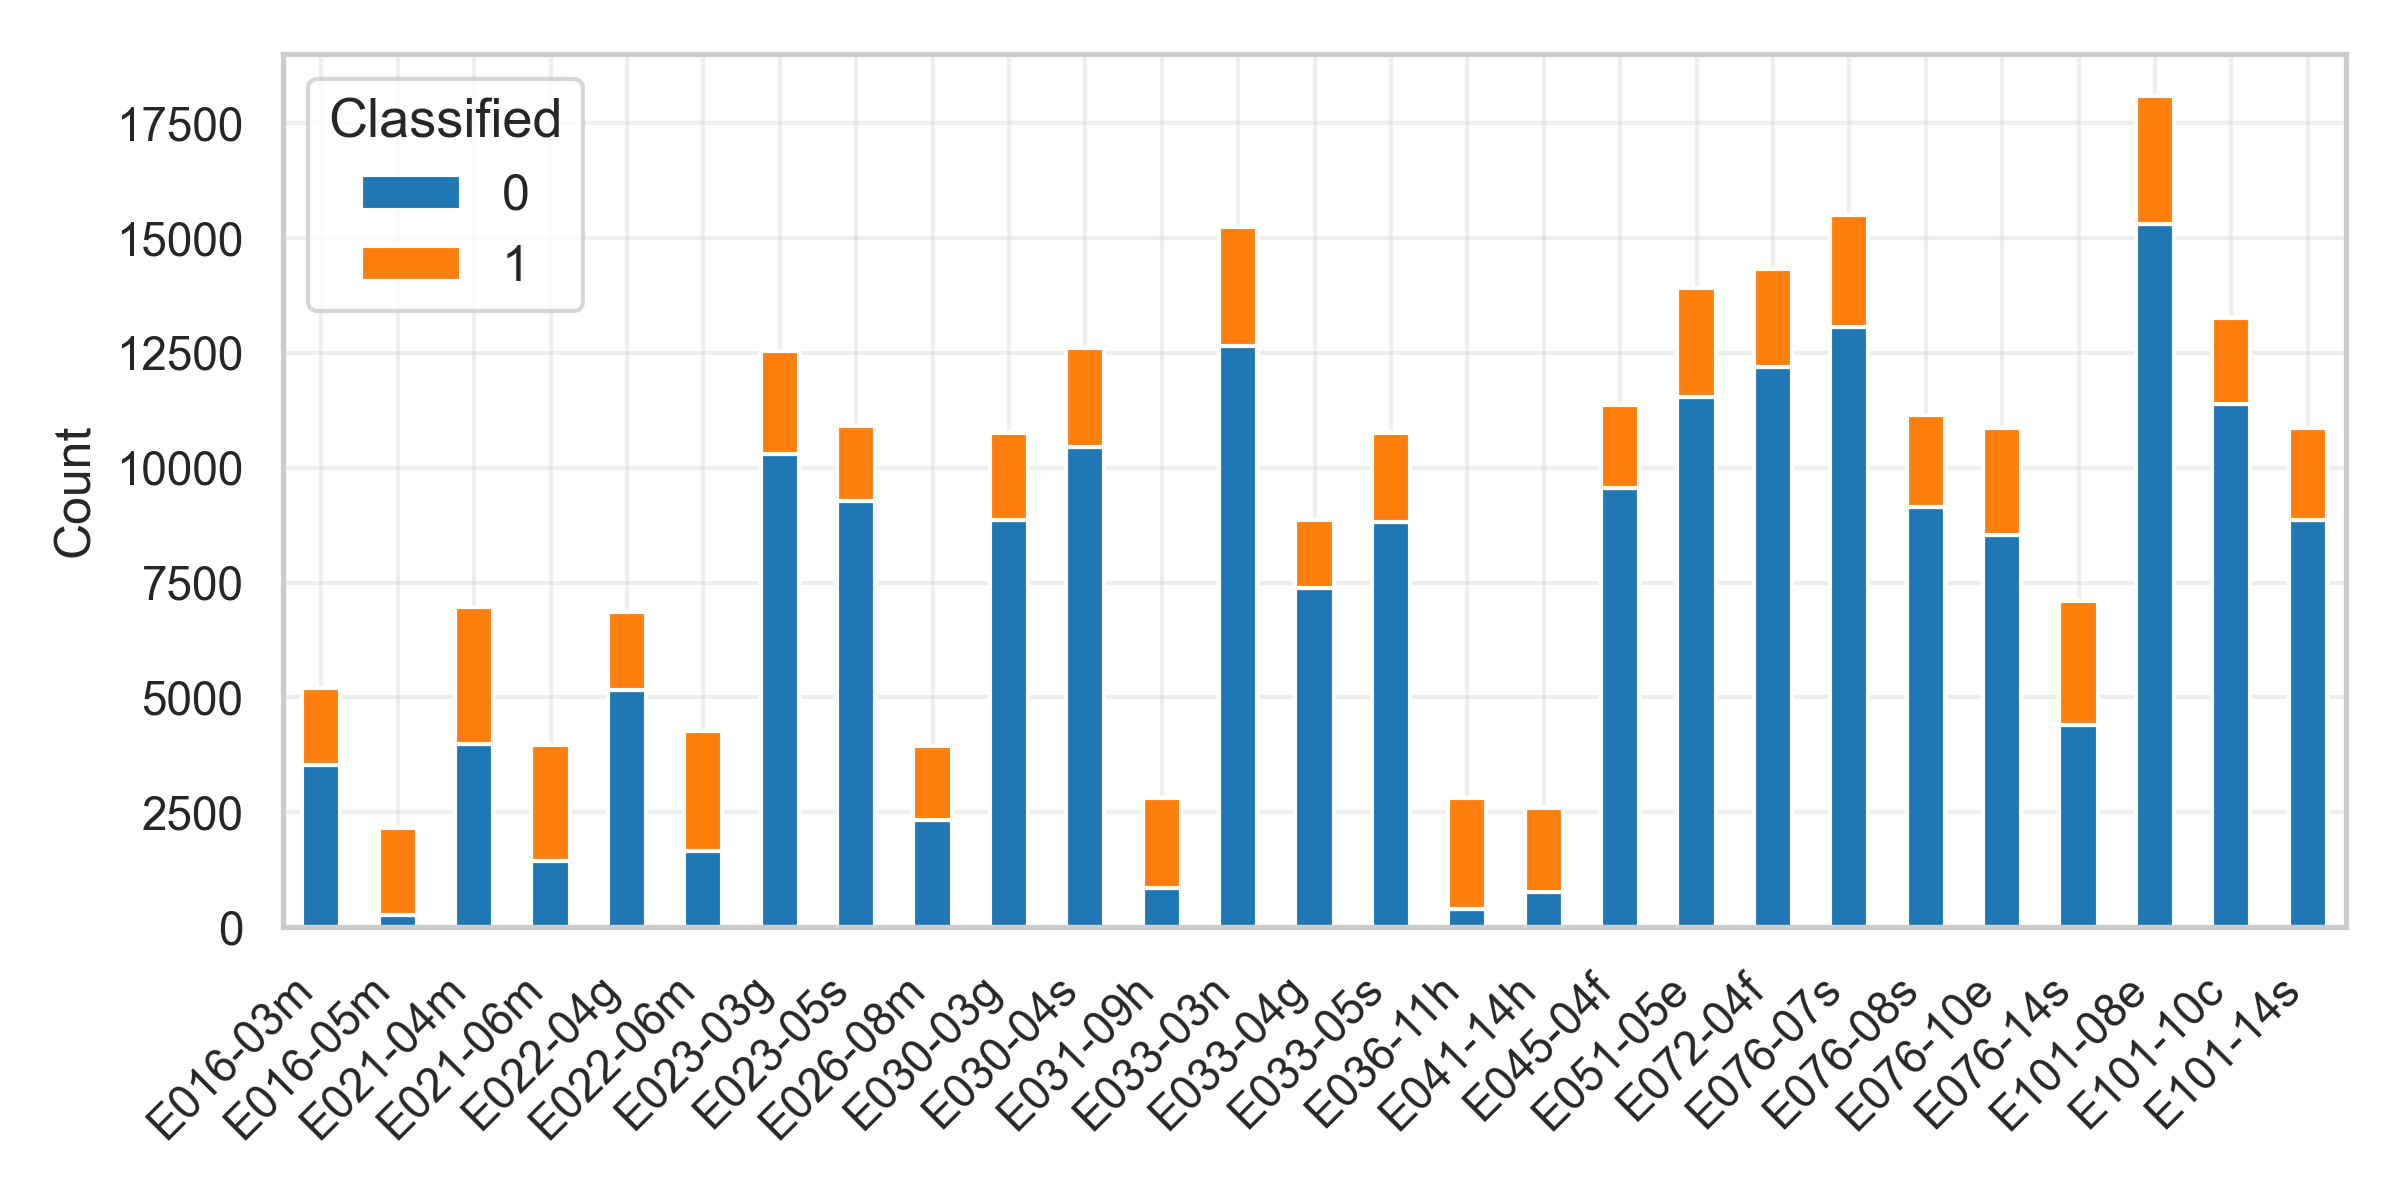
\includegraphics[width=\linewidth]{pictures/dataset_structure/distribution_plot_RandomData_5_40_40_10.png}
        \caption{RD-5-40-40-10.}
    \end{subfigure}%
    \begin{subfigure}[t]{.5\textwidth}
        \centering
        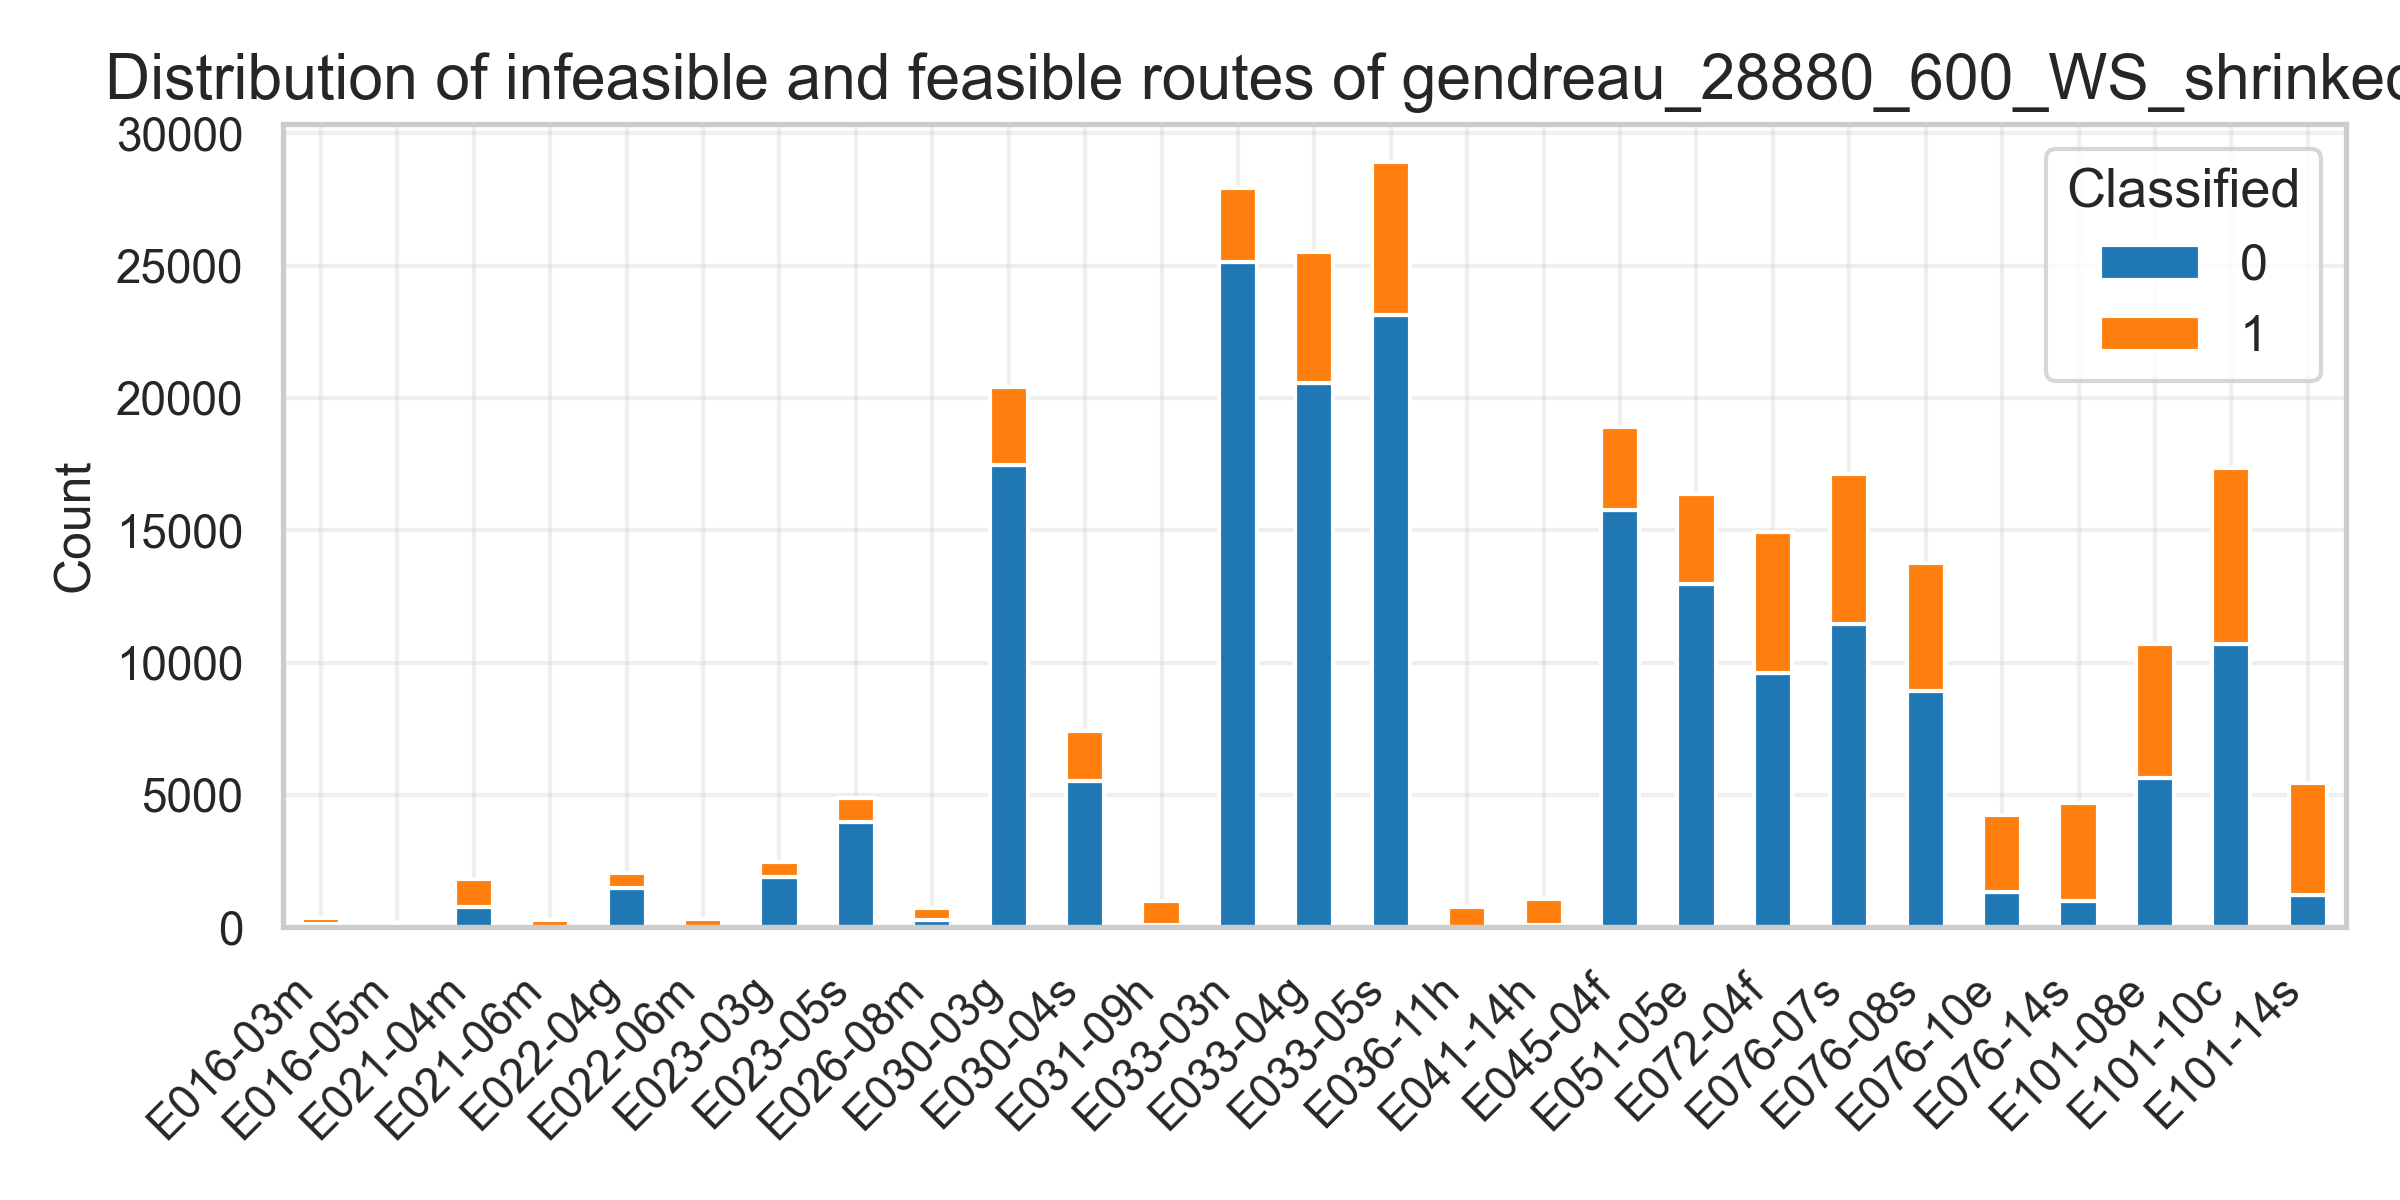
\includegraphics[width=\linewidth]{pictures/dataset_structure/distribution_plot_gendreau_28880_600_WS_shrinked094.png}
        \caption{Complete-WS-Shrinked.}
    \end{subfigure}
    \caption[Distribution of routes considered per instance for two exemplary datasets of random and save strategy.]
    {Distribution of routes considered per instance for two exemplary datasets of random and save strategy.}
    \label{fig:comparison_noroutes_perInstancce}
\end{figure}

\subsection{Feature Filter Results}
\label{sec:feature_filter_results}

The filter algorithm (Algorithm~\ref{alg:filter_algorithm}) was applied using minimum importance thresholds $\epsilon \in {0.1, 0.2, 0.3, 0.4}$
and barrier values $\mathcal{B} \in {0.5, 0.75}$. In addition, Pearson correlation thresholds $\Phi \in {0.8, 0.85, 0.9}$ were considered
across all 27 datasets $\mathcal{D}$ introduced in the previous subsection. Figure~\ref{fig:feature_filter_parameters} in the appendix
illustrates how the drop sets are constructed by varying $\epsilon$ and $\mathcal{B}$. Thresholds below 20\% were also tested but
did not affect the final subsets. The specific features removed under each configuration are listed in Table~\ref{tab:feature_dropsets},
while Table~\ref{tab:drop_set_presentation_shortened} summarizes the drop set names and the number of features excluded. The drop set
names have the following structure: DS-$100\mathcal{B}$-$10\epsilon$. To enable
comparison, an additional empty drop set (DS-0-0) was included.

\begin{table}[ht]
    \centering
    \small
    \begin{tabular}{l c c c c c c c}
        \toprule
        Dropset Name          & DS-0-0 & DS-50-2 & DS-50-3 & DS-50-4 & DS-75-2 & DS-75-3 & DS-75-4 \\
        \midrule
        Barrier $\mathcal{B}$ & -      & 0.5     & 0.5     & 0.5     & 0.75    & 0.75    & 0.75    \\
        Threshold $\epsilon$  & -      & 0.2     & 0.3     & 0.4     & 0.2     & 0.3     & 0.4     \\
        Number Features       & 0      & 10      & 18      & 38      & 7       & 18      & 32      \\
        \bottomrule
    \end{tabular}
    \caption{Presentation of the considered drop sets for the feature selection.}
    \label{tab:drop_set_presentation_shortened}
\end{table}
For each drop set, every dataset was trained with each model type and then used to predict the
true labels of all other datasets in order to identify the best-performing drop set. The hyperparameters used for
each model are provided in Table~\ref{tab:hyperparams_feature_selection} in the appendix. For the subsequent analysis,
results obtained from predicting between datasets of the save strategy were excluded, since these datasets are nested
subsets of one another (see Table~\ref{tab:saved_instances_gendreau}). Figure~\ref{fig:mcc_filter_results} presents boxplots of
the \gls{MCC} for all drop sets and the three model types introduced in Section~\ref{sec:modelselection}.

\begin{figure}[ht]
    \centering
    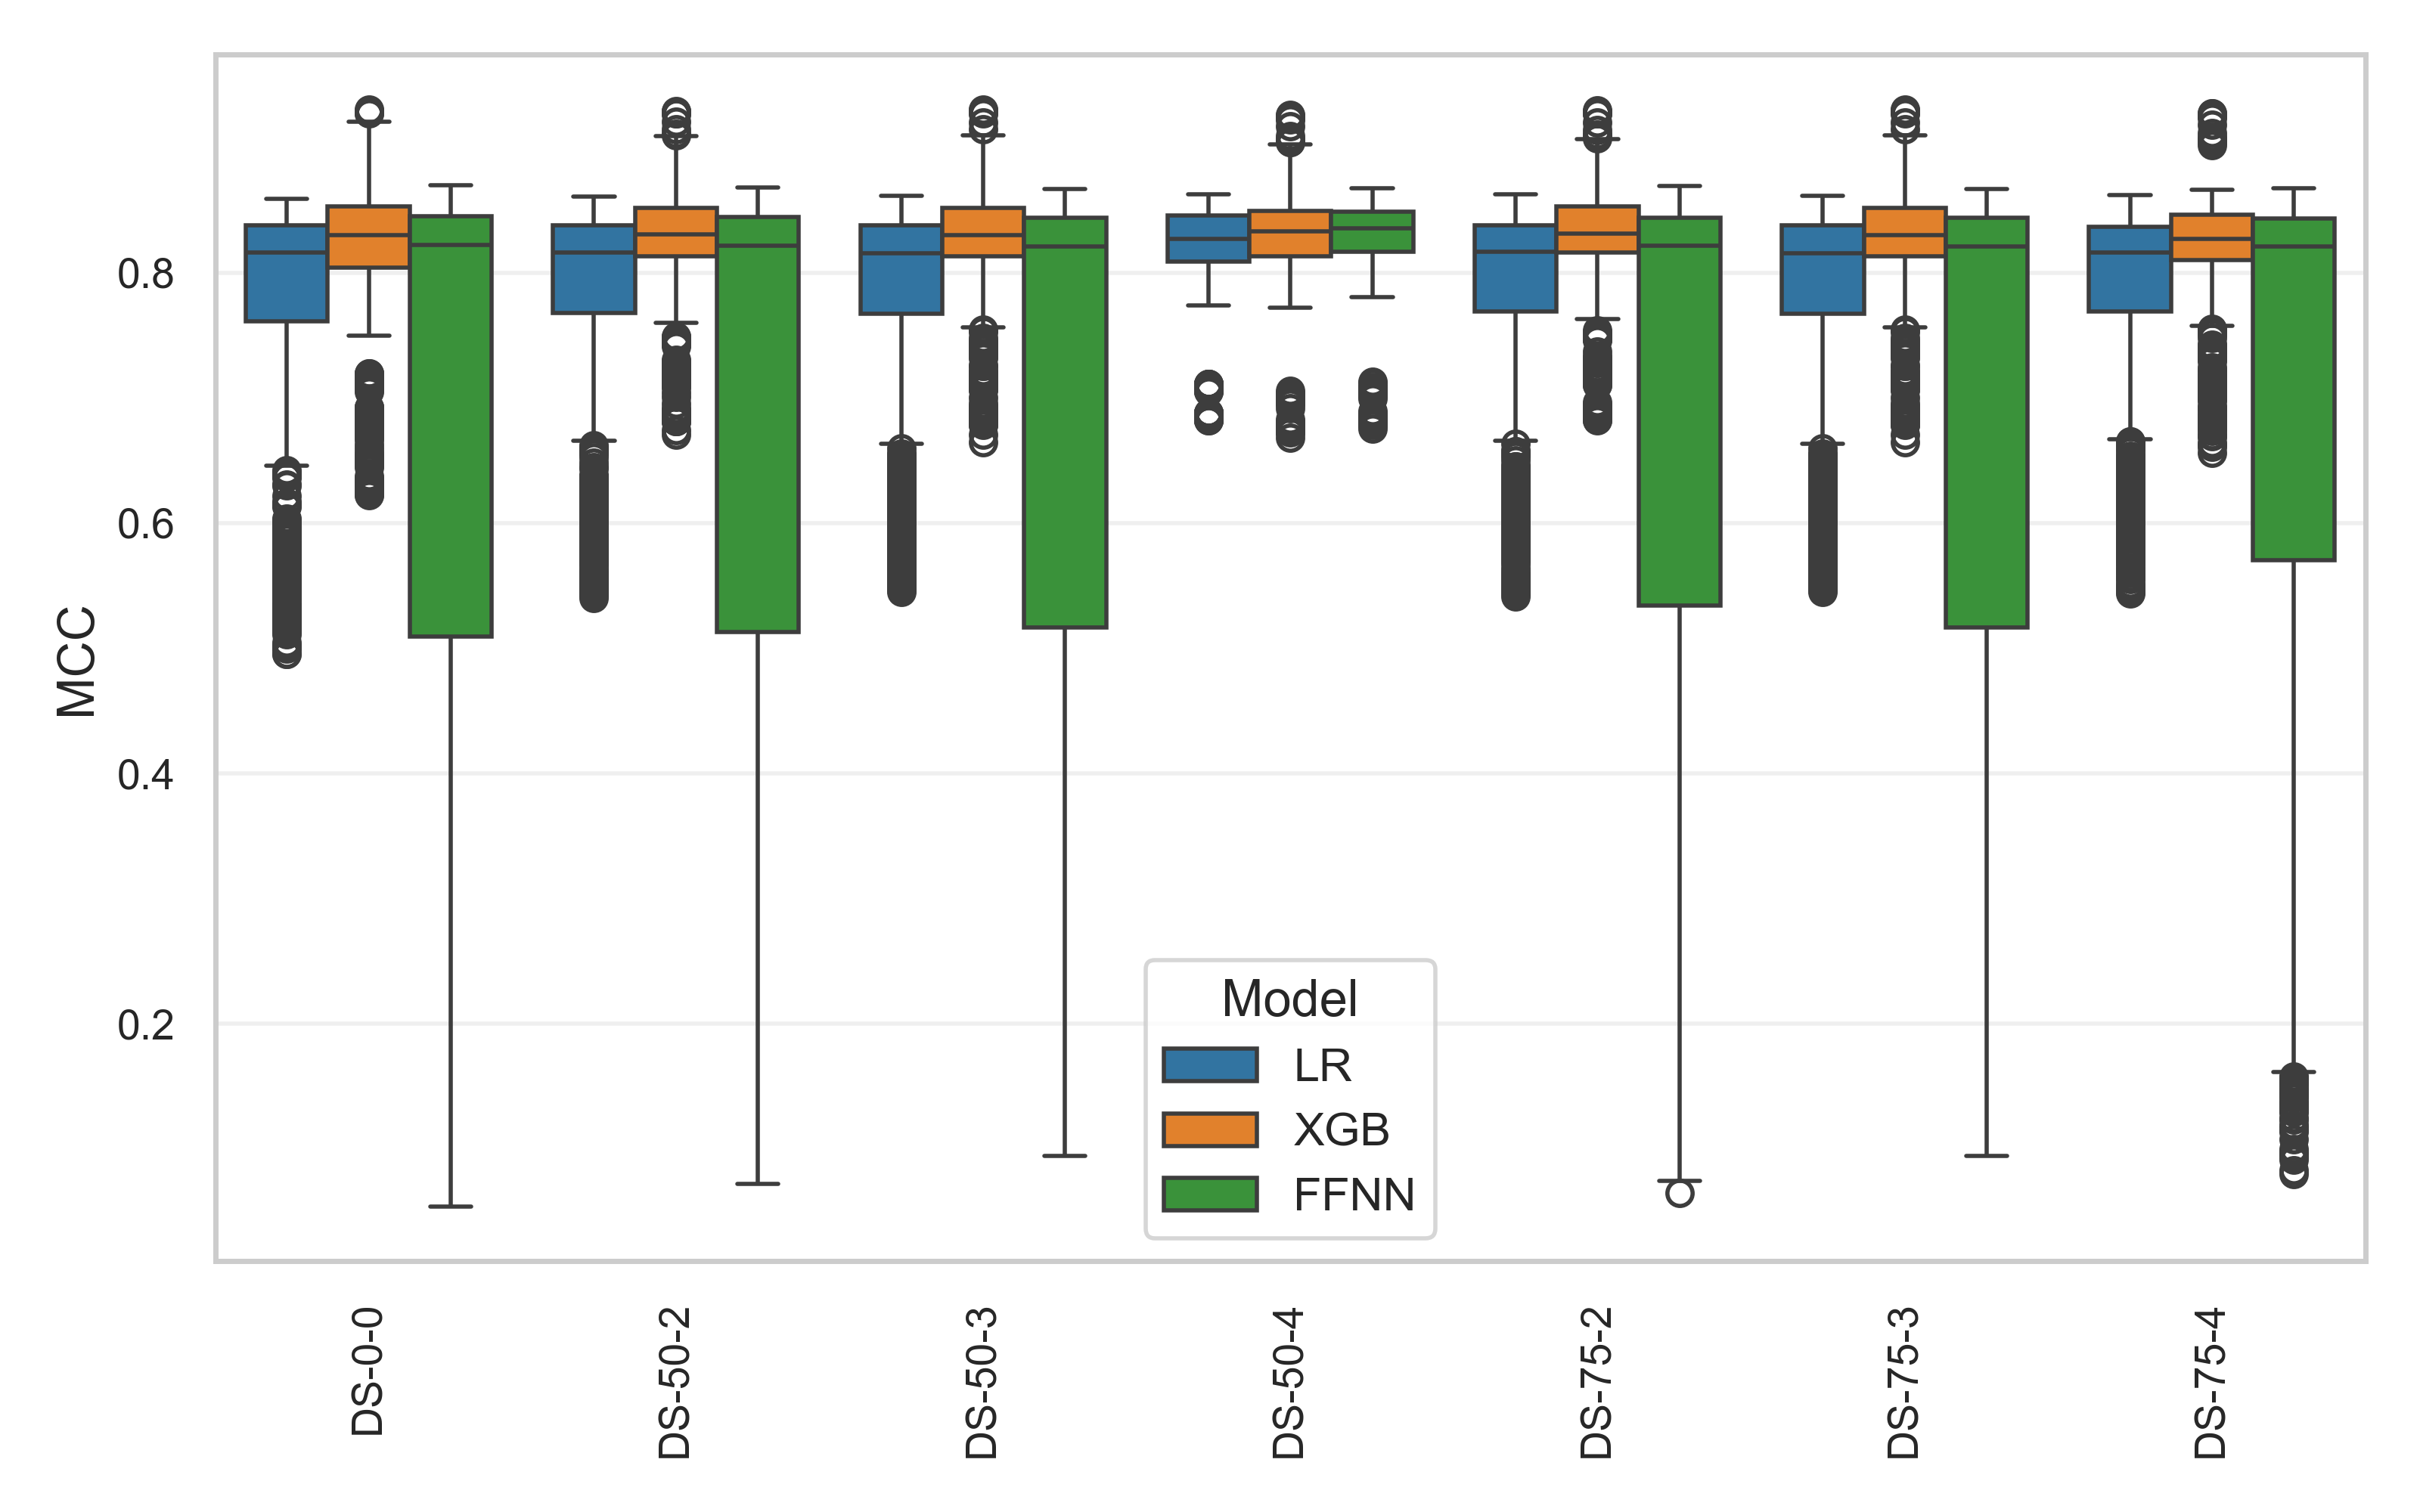
\includegraphics[width = .85\textwidth]{pictures/feature_filter/all_data_exceptSubsets_box_plot.png}
    \caption{Box plots of MCC performance of different feature drop sets.}
    \label{fig:mcc_filter_results}
\end{figure}
Two main observations can be drawn from the boxplot. First, the FFNN exhibits the widest variation in performance, whereas the XGB model
shows the smallest. Second, dropset DS-50-4 achieves the most consistent results across datasets. For both LR and FFNN, the performance
spread is larger than for XGB due to the need to scale the data before making predictions. Since scaling depends on the statistics of
the training dataset (e.g., mean and standard deviation), differences in dataset structure\footnote{Compare Table~\ref{tab:saved_instances_gendreau} and Table~\ref{tab:created_instances_xyz_gendreau} for the created datasets.}
can lead to mismatched feature ranges in the prediction datasets, thereby reducing performance. The FFNN is particularly sensitive
to such mismatches, as the hidden layers amplify these effects more strongly than in LR. Dropset DS-50-4, which removes 38 of
the 48 initial features, mitigates this issue by reducing complexity and minimizing the risk of mis-scaling, while still
achieving predictive performance comparable to other drop sets, as seen in the boxplot comparison. The full set of results across
all performance metrics is presented in Table~\ref{tab:featurePerformance_Alldata}.

\begin{table}[ht]
    \centering
    \small
    \begin{tabular}{lrrrrrrr}
        \toprule
        DropSet  & DS-0-0 & DS-50-2 & DS-50-3 & DS-50-4       & DS-75-2 & DS-75-3 & DS-75-4 \\
        \midrule
        MCC      & 0.75   & 0.76    & 0.76    & \textbf{0.82} & 0.76    & 0.76    & 0.76    \\
        F1-Score & 0.81   & 0.82    & 0.82    & \textbf{0.88} & 0.82    & 0.82    & 0.82    \\
        Accuracy & 0.89   & 0.89    & 0.89    & \textbf{0.93} & 0.89    & 0.89    & 0.89    \\
        AUROC    & 0.96   & 0.96    & 0.96    & \textbf{0.98} & 0.95    & 0.96    & 0.96    \\
        \bottomrule
    \end{tabular}
    \caption[Mean performance metrics on various different drop set excluding the predicting between save strategy datasets.]
    {Mean performance metrics on various different drop set excluding the predicting between save strategy datasets.
        Bold font shows the best results for each performance score.}
    \label{tab:featurePerformance_Alldata}
\end{table}

The final features considered for predicting the loading feasibility are the following:
\begin{table}[!ht]
    \centering
    \def\arraystretch{1.5}
    \begin{tabular}{l l l l }
        \sbt Rel Volume      & \sbt Fragile Sequence    & \sbt width-W-mean & \sbt height-H-std    \\
        \sbt  length-L-std   & \sbt Weight Distribution & \sbt width-W-std  & \sbt height-area-min \\
        \sbt  area-AREA-mean & \sbt area-AREA-max       &                   &                      \\
    \end{tabular}
\end{table}

Additional feature filter results are provided in Section~\ref{app:sec:further_feature_filter} of the appendix.
These confirm that drop set DS-50-4 achieves the best overall performance, while models requiring feature scaling generally perform worse
across multiple datasets. The following section addresses the selection of datasets to be used as classifiers in the final algorithm.

\subsection{Selection of dataset}
\label{sec:dataset_selection}

The feature filter performance analyses described in the previous section can be used to identify the best-performing datasets
from each retrieval strategy, when results are filtered for drop set DS-50-4. Figure~\ref{fig:dataset_performance_group_subgroup}
shows the MCC performance as a function of the chosen base dataset (Group) and the subgroup of predicted datasets, which are either
random or save-strategy datasets. Here BC stands for the save strategy with the B\&C algorithm.
As noted earlier, for save-strategy datasets only the performance on the base dataset is considered,
since these datasets are nested subsets of one another.
\begin{figure}[ht]
    \centering
    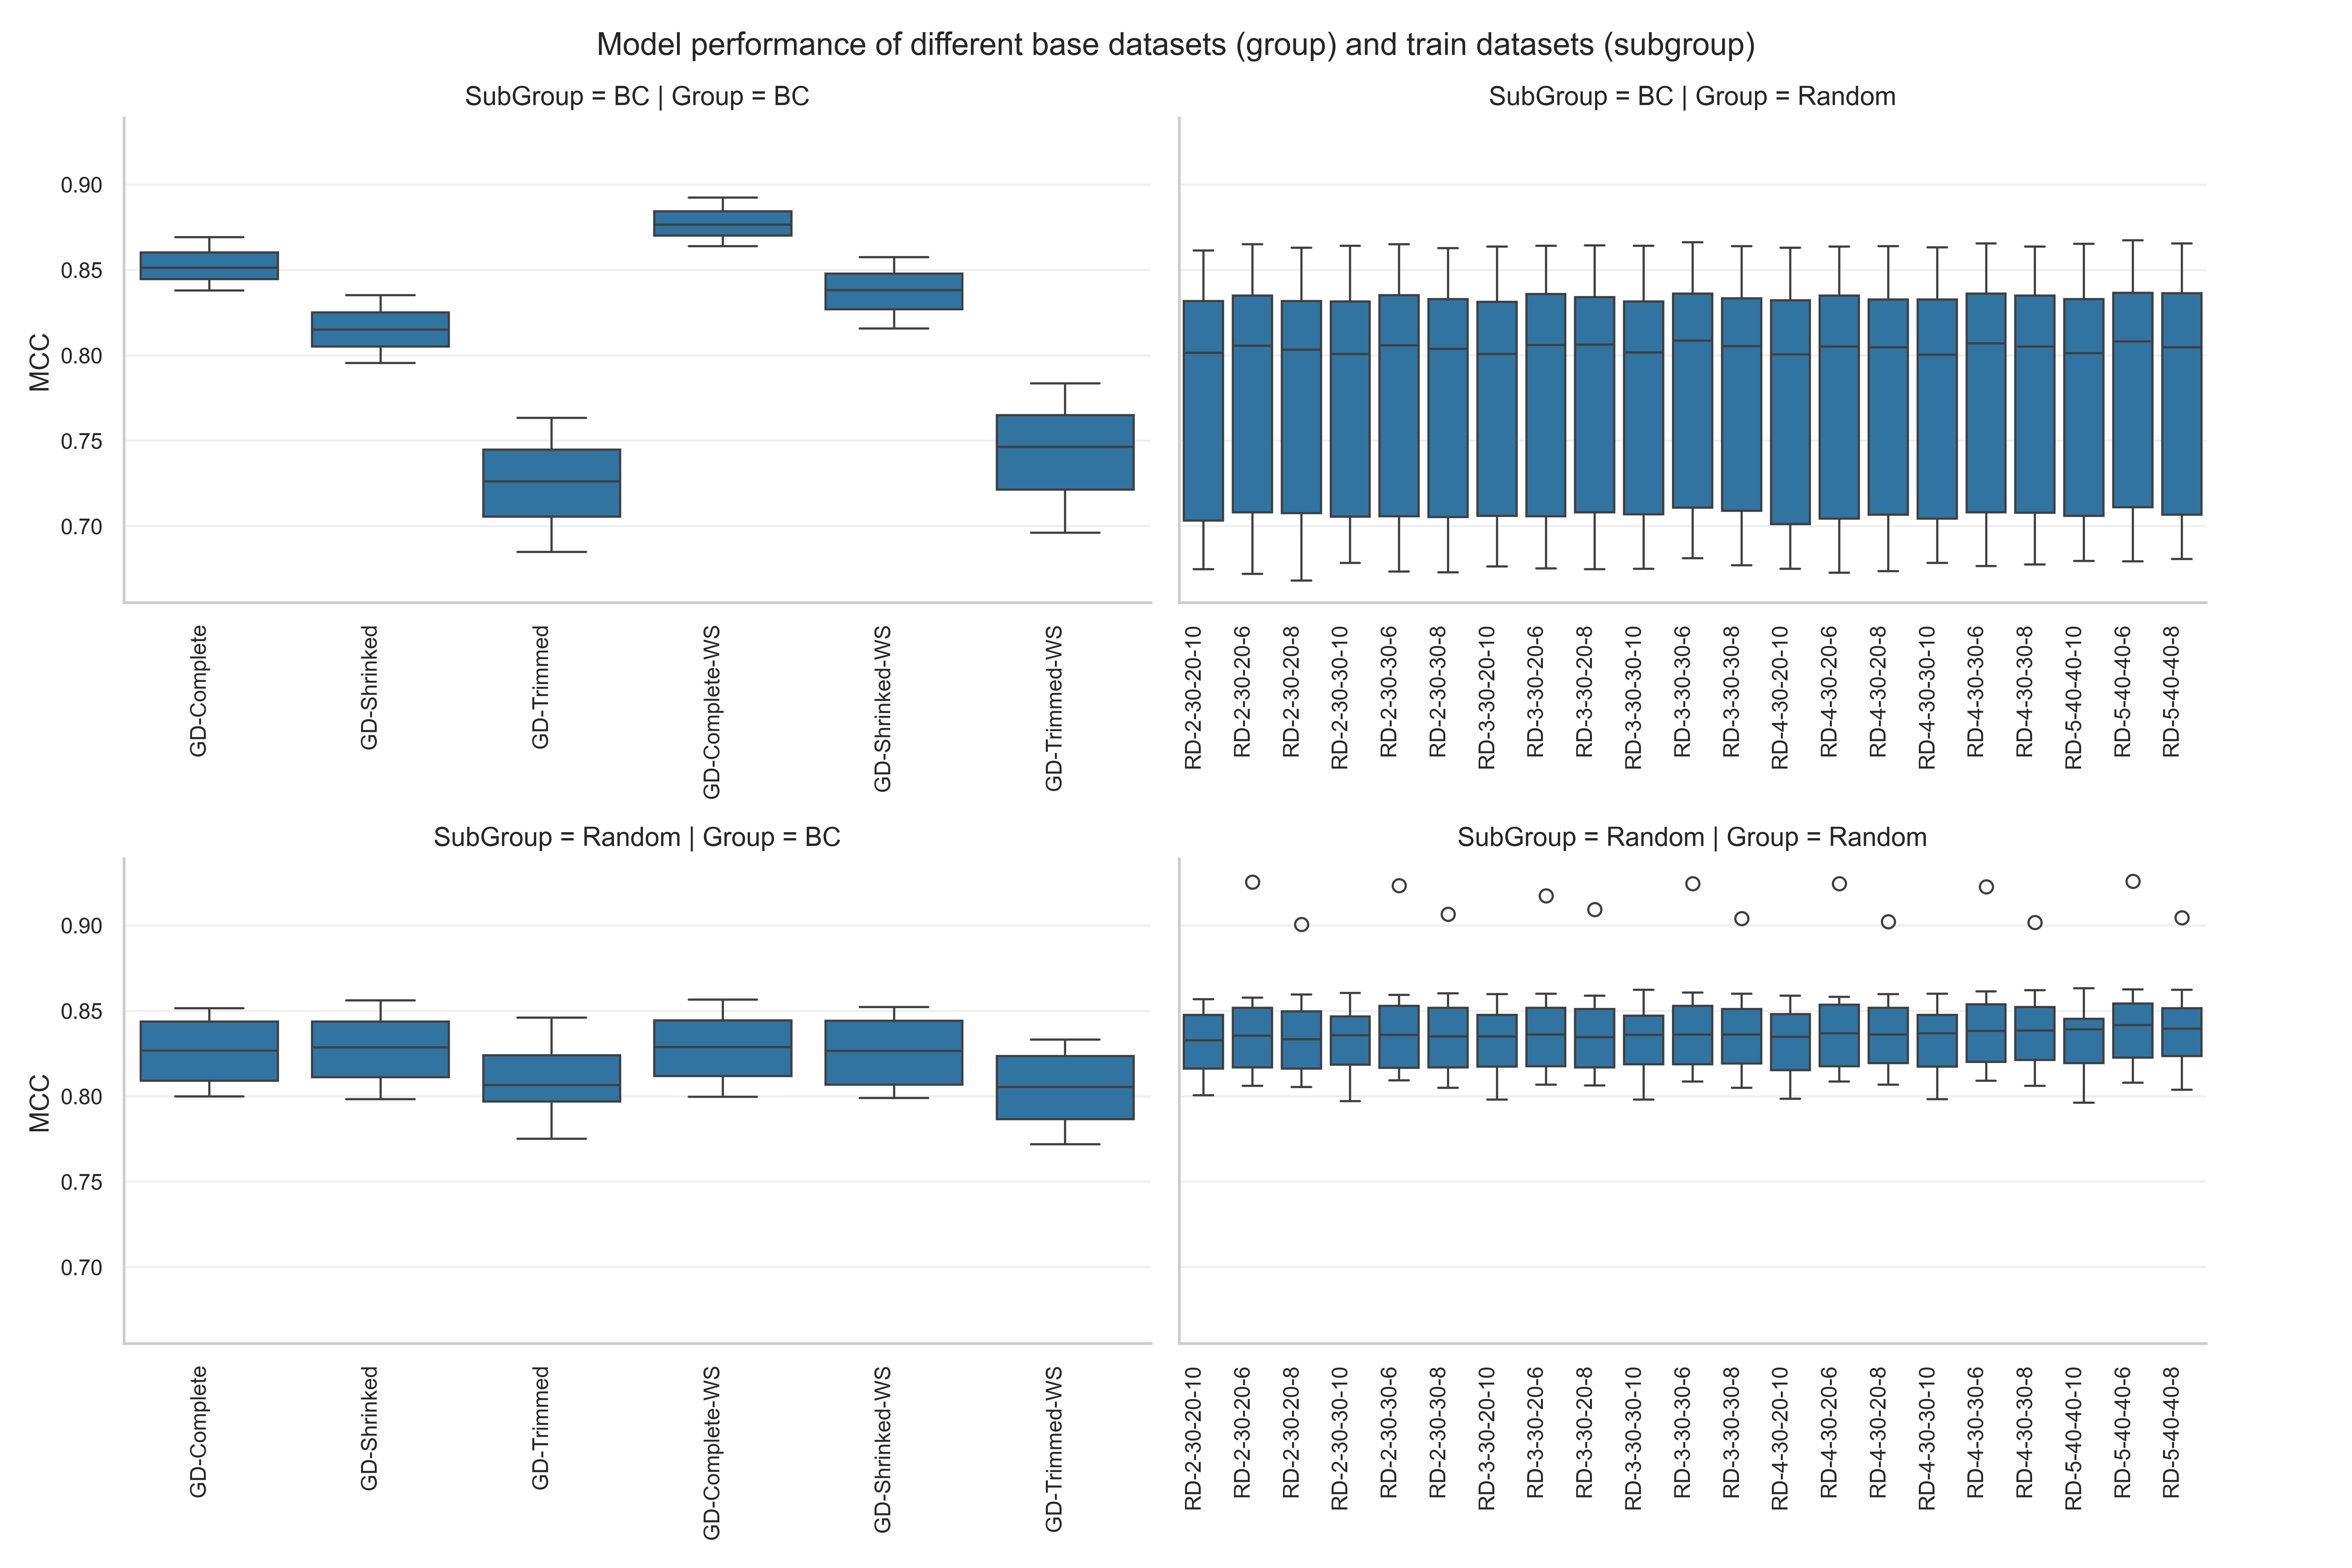
\includegraphics[width =\textwidth]{pictures/feature_filter/group_subgroup_results.png}
    \caption{Box plots of MCC performance of different feature drop sets.}
    \label{fig:dataset_performance_group_subgroup}
\end{figure}

In the first subplot, where Group = SubGroup = BC, only the performance on the base training dataset is
displayed for each respective model type (\gls{LR}, XGB, and \gls{FFNN}). This subset is the only one showing significant
performance differences, with the Complete datasets outperforming the others. When the subgroup consists of random datasets,
the performance of the Shrinked and Complete datasets is similar. The Trimmed datasets, however, can be excluded from consideration,
as their predictive capability is restricted by the lack of feasible small tours (only infeasible two-customer routes are included).
For the random dataset subgroup, the results are more difficult to interpret, as the median performance remains nearly constant
across datasets. Still, when both group and subgroup are random datasets, a slight improvement in median performance can
be observed for smaller values of $\delta$ within the same ($\alpha$, $\beta$, $\gamma$) group. To avoid arbitrary dataset
selection, an additional validation dataset was constructed by saving the routes found during the base \gls{ILS} algorithm,
with feasibility checks carried out exclusively by the \gls{CP} solver. Each instance from \gendreauDataSetText was run
five times with different seeds and an extended time limit of 15 minutes to generate a large set of candidate routes.
The parameters used for this run are provided in Table~\ref{tab:parameters_final_noclassifier} in the following section and
the validation dataset characteristics in the Table~\ref{tab:validation_dataset_gendreau}.
\begin{table}[!h]
    \centering
    \small
    \begin{tabular}{l c c c c c }
        \toprule
        Name          & Routes & Route Len = 2 & Balance   & Rel. Vol & Rel. Mass \\
        \midrule
        Validation DS & 427048 & 8605          & 47.0/53.0 & 0.61     & 0.60      \\
        \bottomrule
    \end{tabular}
    \caption{Validation dataset characteristics constructed from \gendreauDataSetText with ILS algorithm.}
    \label{tab:validation_dataset_gendreau}
\end{table}

The datasets contains many rows with a balanced profile of feasible and infeasible labels. In comparison to both
random and save strategy datasets the number of routes with two customers is very low, as the \gls{ILS} algorithm
works with dense routes to improve the solution quality. The \gls{MCC} score for every model and train dataset
from random and save strategy is shown in the following Figure~\ref{fig:validation_performance_line_plot}.

\begin{figure}[ht]
    \centering
    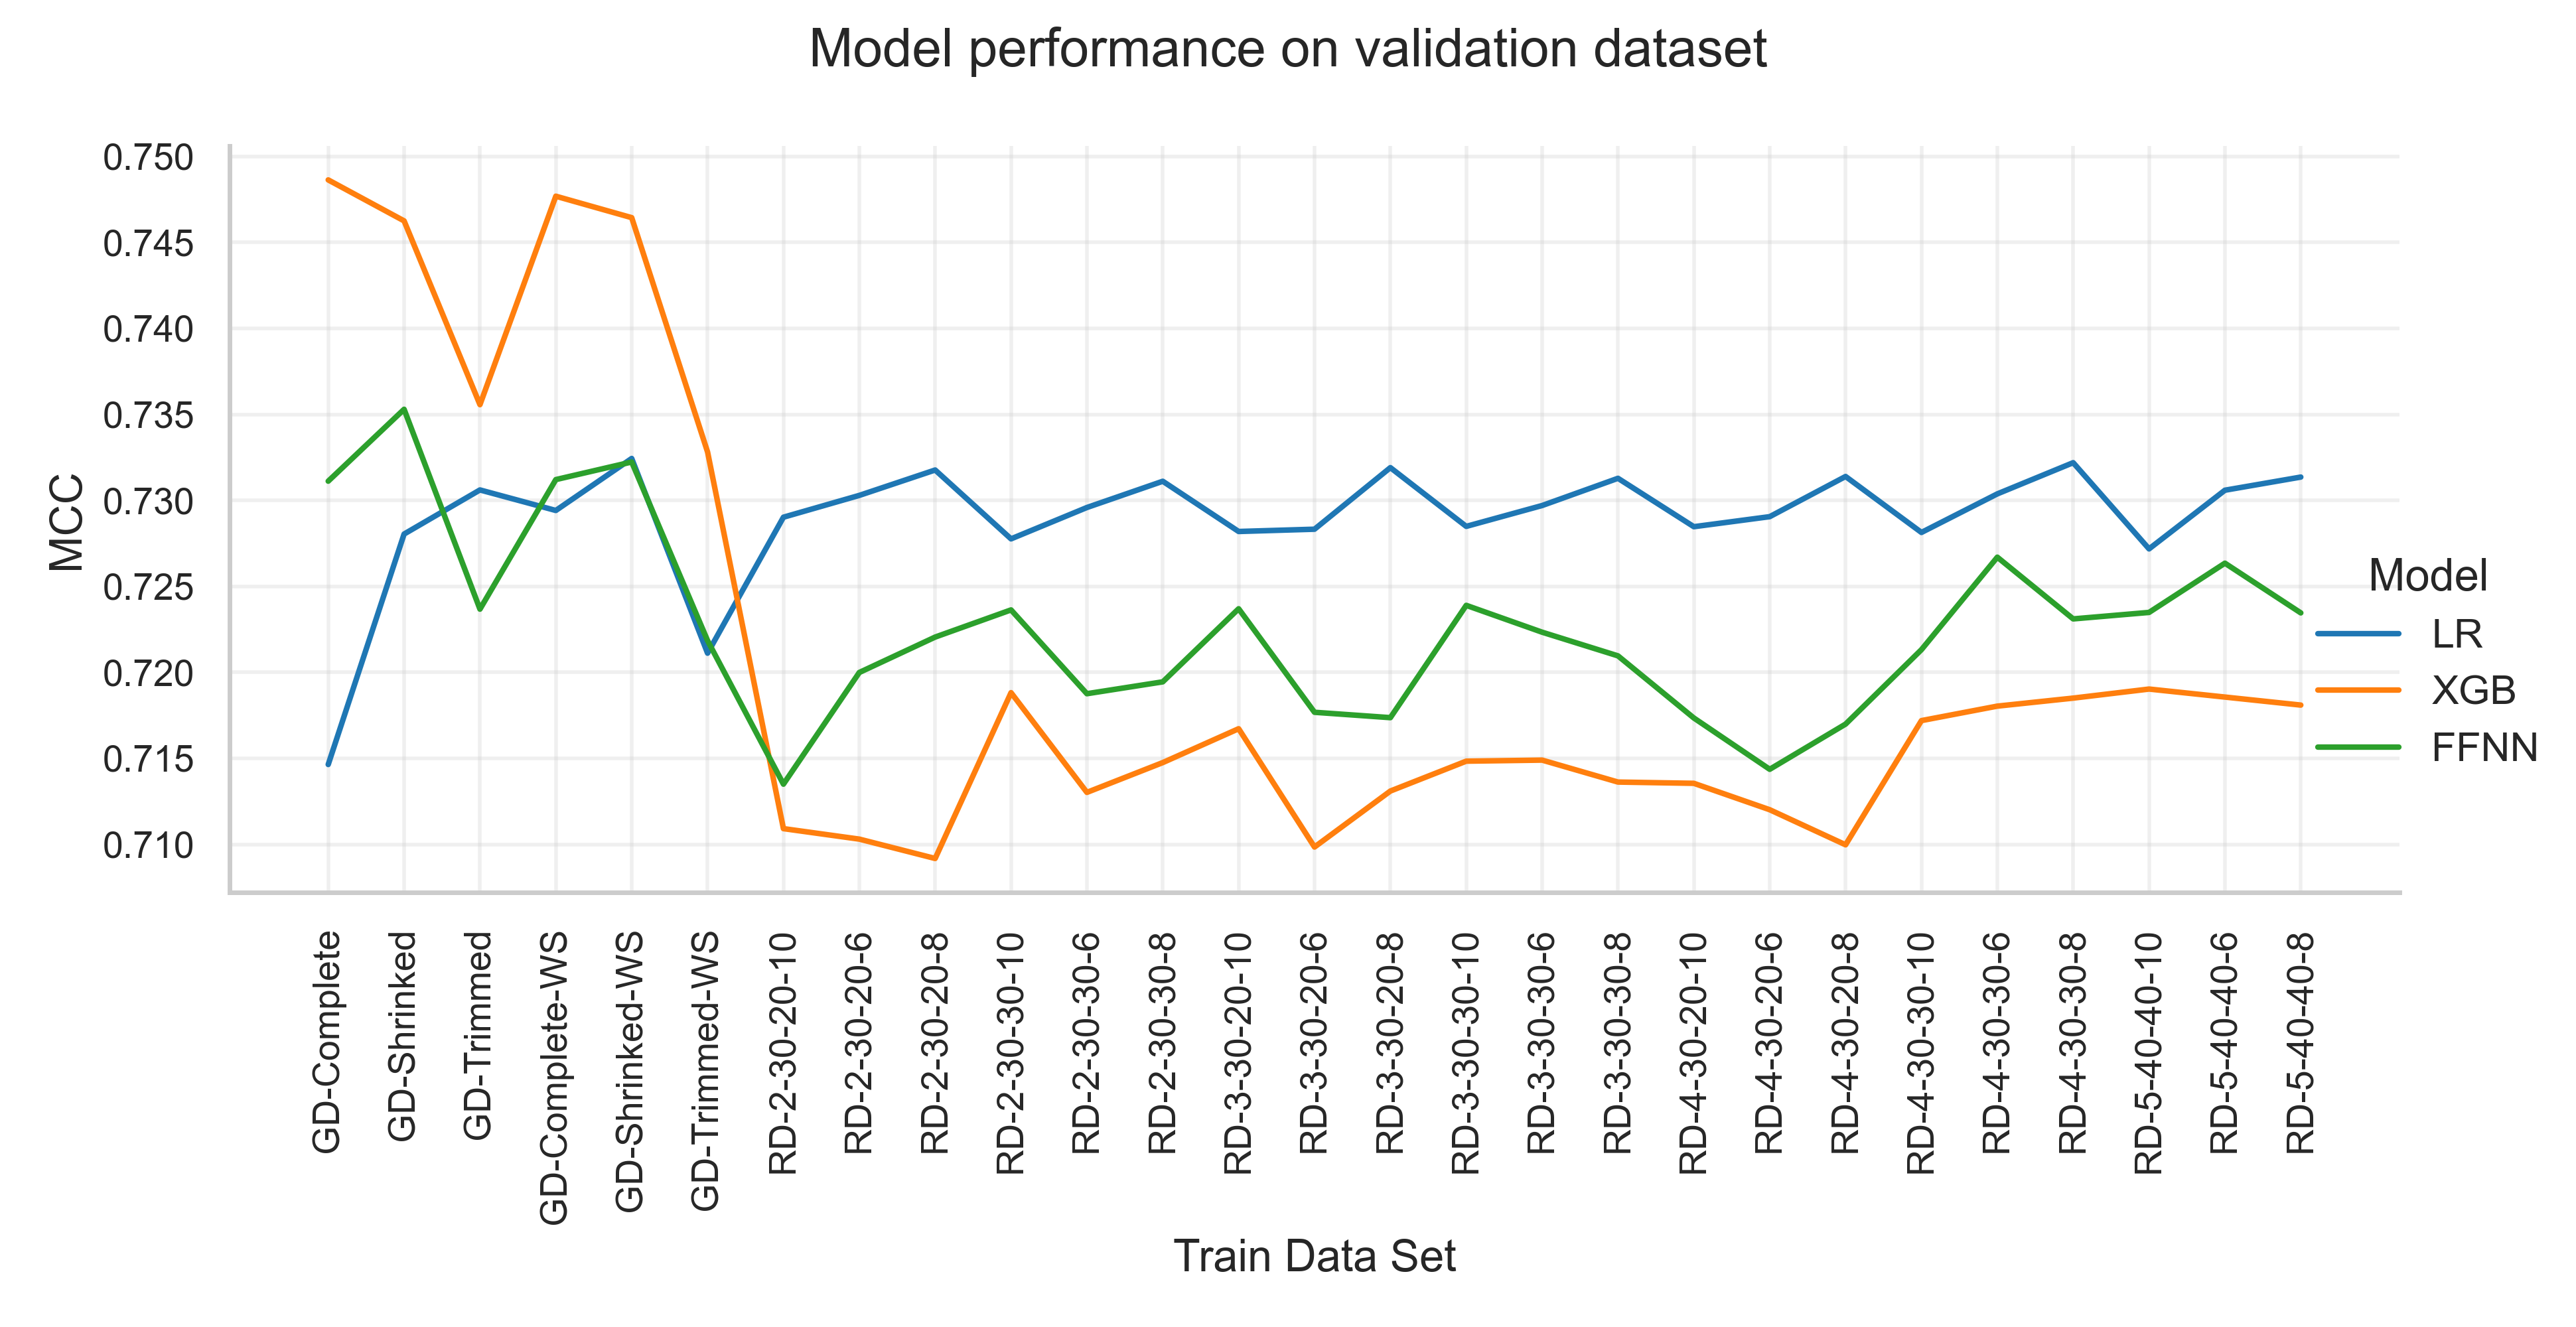
\includegraphics[width =\textwidth]{pictures/feature_filter/validation_line_plot.png}
    \caption{Obtained MCC from validation dataset based on different train datasets and model types.}
    \label{fig:validation_performance_line_plot}
\end{figure}

With the exception of the trimmed datasets, the save-strategy datasets generally achieve better predictive performance.
However, the MCC scores, independent of the training dataset, are significantly lower than those shown in
Figure~\ref{fig:dataset_performance_group_subgroup}. While the LR model yields consistent values across dataset groups,
the performance of XGB and FFNN decreases when trained on random-strategy datasets, reversing the ranking of the best-performing
models from one group to the other. This motivates a more detailed comparison of solution quality with respect to dataset type and
its causal relationship with model choice. The complete results for all performance metrics are reported in Table~\ref{tab:featurePerformance_validationDataset},
with the best values highlighted in bold. The choice of the two datasets is based on their superior performance among the evaluation metrics,
but also on the need to compare random versus save-strategy datasets and to examine whether adjusting the threshold $\delta$ or adding
more routes to the training dataset (WS) yields better results.

\begin{table}[ht]
    \centering
    \setlength{\tabcolsep}{0.75em}
    \def\arraystretch{1.5}
    \begin{tabular}{l|ll}
        Save Strategy   & GD-Shrinked  & GD-Shrinked-WS \\\hline
        Random Strategy & RD-4-30-30-6 & RD-4-30-30-8   \\
    \end{tabular}
    \caption{Chosen datasets for training final classifier.}
    \label{tab:chosen_datasets}
\end{table}

\section{Parameter Study}
\label{sec:parameter_study}

The parameter study is divided in four subsections following the variants of the algorithm
presented in Section~\ref{sec:FeasibilityCheck}. This study follows a hierarchical procedure
tuning the parameters, introduced for each variant, sequentially. The following subset of 13
instances from \gendreauDataSetText is used:


\begin{table}[ht]
    \centering
    \setlength{\tabcolsep}{0.75em}
    \def\arraystretch{1.5}
    \begin{tabular}{lllllll}
        E016-03m & E022-04g & E023-03g & E023-05s & E030-03g & E033-04g & E033-05s \\
        E051-05e & E072-04f & E076-07s & E076-14s & E101-10c & E101-14s &          \\
    \end{tabular}
\end{table}

The division followed the following approach, first all instances were omitted, which found
the optimal solution in a short time (see \cite{tamke_branch-and-cut_2024}\footcite[cf.][p.26]{tamke_branch-and-cut_2024}).
Second, similar instances of size and complexity were reduced to only one.
Every instance is run three times with different seeds and a timelimit of 10 min. It will be investigated
how different parameter combinations influence the \gls{RDP}, the iteration number, the rejection rate and
the average improvement per second after finding the initial solution. The \gls{RDP} is defined between the
total costs of the best solution $C^*$ and another solution with costs $C$.
\begin{align}
    RPD = \frac{C - C^*}{C^*} \cdot 100\%
\end{align}
The rejection rate is the proportion of iterations rejected as infeasible in the \gls{CP} check, which needs
to be applied after the \textit{SpeedUp} and \textit{Hybrid} variant. These variants allow the acceptance of
new solutions only based on the classification and need to be checked for \gls{FP} routes afterwards.
All experiments were run on a AMD EPYC 7513 32-Core machine with 8 cores maximum available for the \gls{CP} solver
The \gls{ILS} algorithm is implemented in C++ and all models were pretrained in Python and loaded afterwards in
the metaheuristic.

\subsection{NoClassifier Variant}
\label{subsec_parameterStuy_noclassifier}
In this variant, all base \gls{ILS} parameters are tested, providing the foundation for subsequent variants,
with the limitation that loading is checked only using the exact \gls{CP} solver. The following levels of
different parameters were selected in a full grid parameter study.
\begin{table}[ht]
    \centering
    \setlength{\tabcolsep}{2em}
    \def\arraystretch{1.1}
    \begin{tabular}{@{}L{4cm}P{8cm}@{}}
        \toprule
        Parametertype      & Levels                                                         \\
        \midrule
        AttemptsLimit $a$  & 3, 5, 8, 12                                                    \\
        RandomMoves R      & 2, 4, 8, 12                                                    \\
        Perturbation       & R-Swaps, R-Insertions, Both-Insertions-First, Both-Swaps-First \\
        Neighborhood order & IntraFirst, InterFirst                                         \\
        \bottomrule
    \end{tabular}
    \caption{Parameter levels for NoClassifier variant.}
    \label{tab:parameters_noclassifier}
\end{table}
The core result is that the \gls{ILS} without speedups relies heavily on the number of iterations to find high-quality solutions.
For some instances, the average number of ILS iterations is very low, as shown in Figure~\ref{fig:average_iterations_noclassifier}.
To account for this, the instances were divided into two groups depending on whether the average number of iterations was below 25
(visualized with different bar colors and the horizontal red line). The heatmap of the parameters RandomMoves and LimitNoImpr
(Figure~\ref{fig:heatmap_parameter_study}) indicates that the best solutions were found either when very few perturbations were
executed or when the search was frequently reset to the best solution found so far, thereby limiting the number of intensification
phases starting from a strongly perturbed solution.
\begin{figure}[ht]
    \centering
    \begin{minipage}[t]{0.49\textwidth}
        \centering
        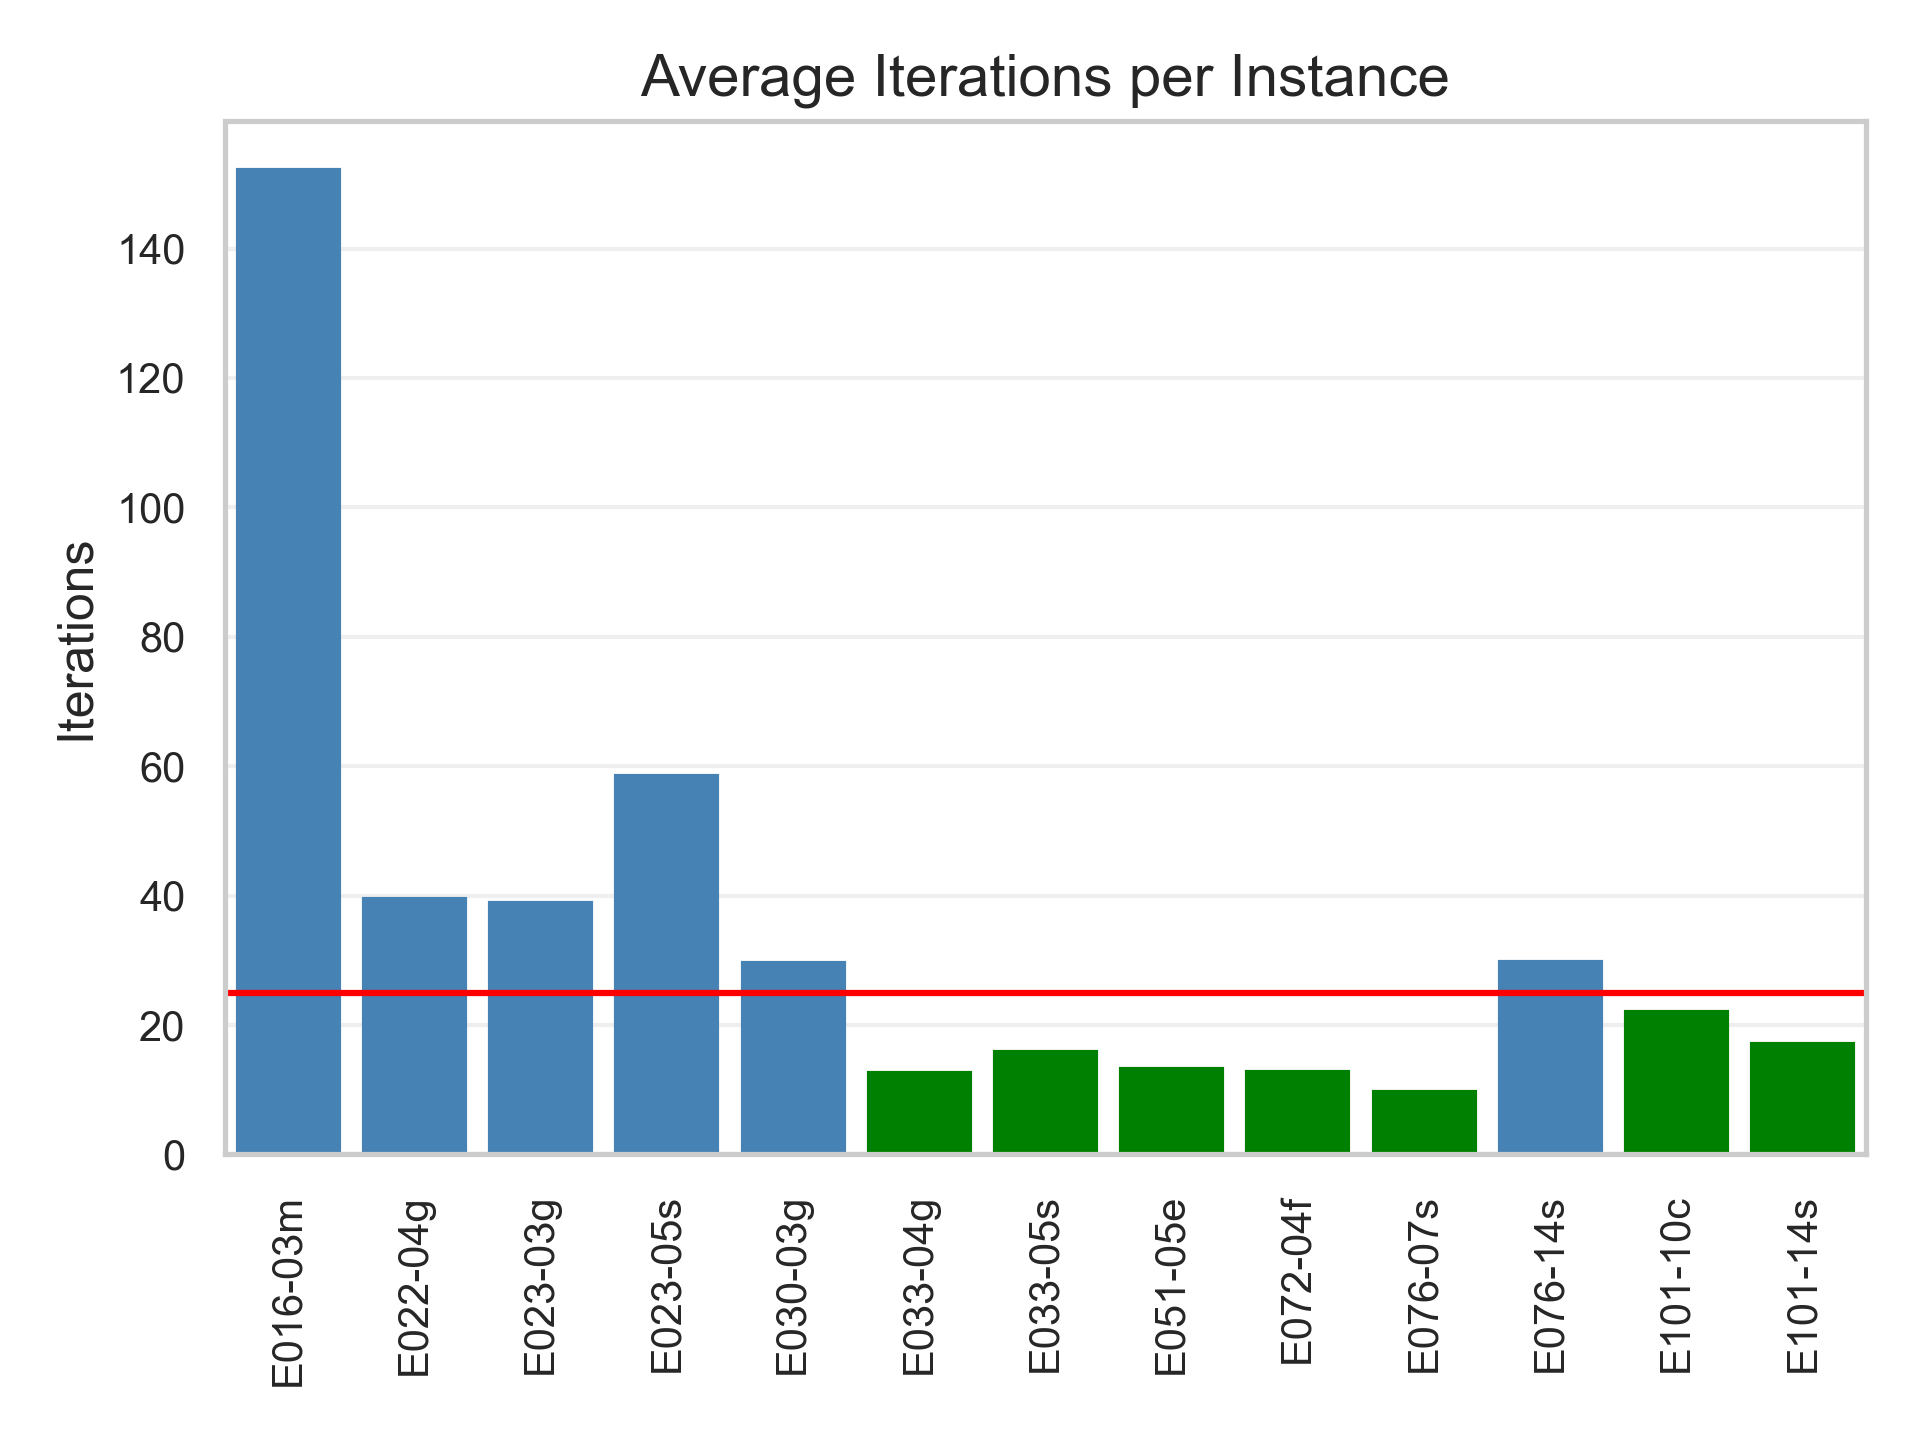
\includegraphics[width=\linewidth]{pictures/iterations_per_instance.png}
        \captionof{figure}{\small Average iterations for each \gendreauDataSetText instance.}
        \label{fig:average_iterations_noclassifier}
    \end{minipage}\hfill
    \begin{minipage}[t]{0.49\textwidth}
        \centering
        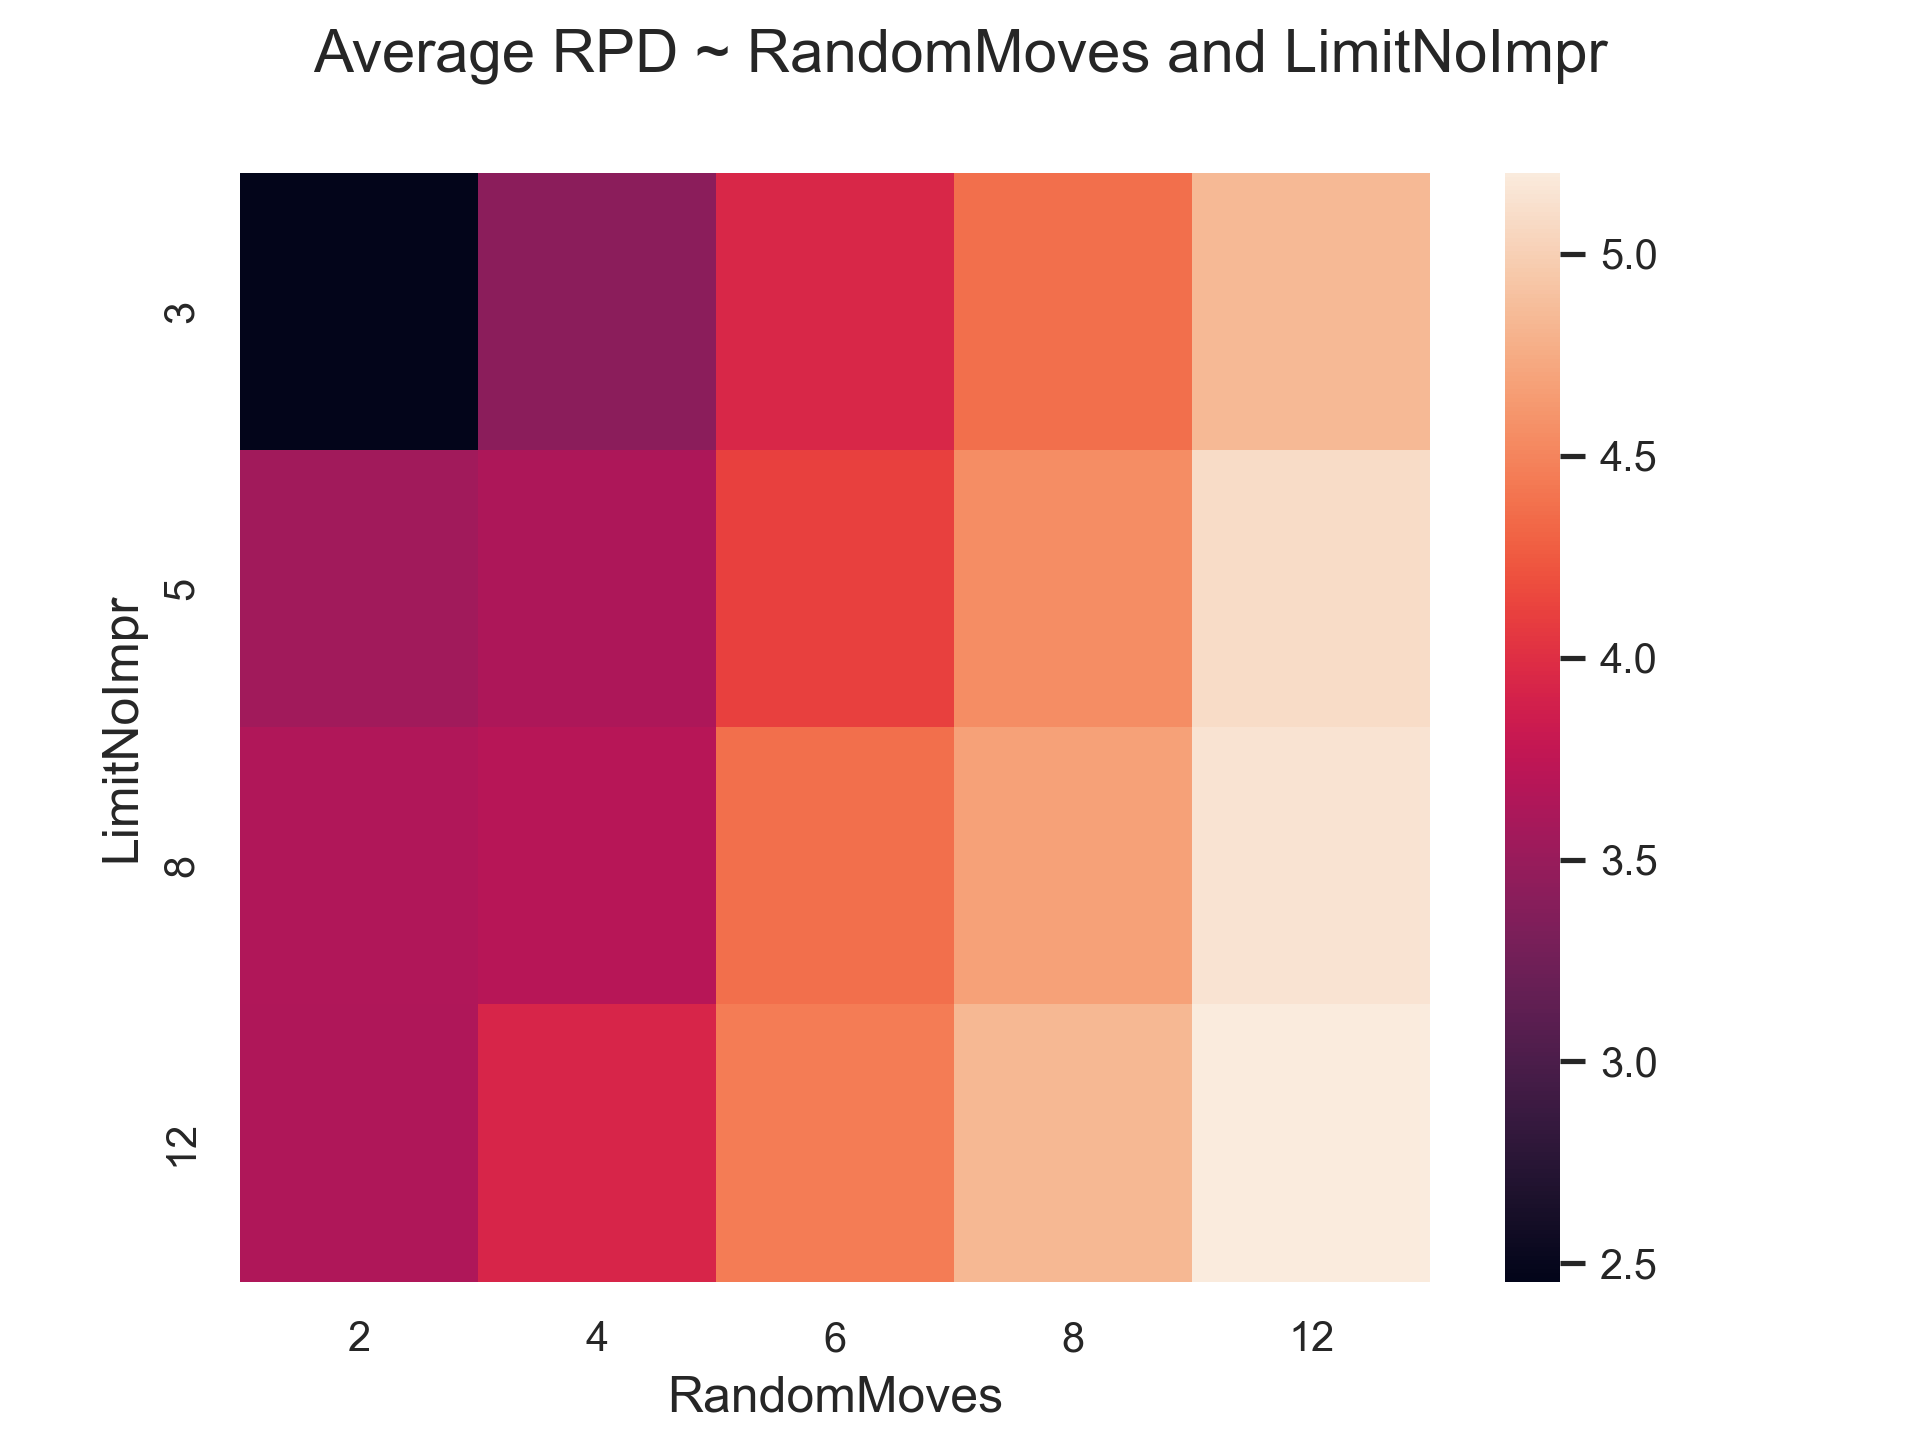
\includegraphics[width=\linewidth]{pictures/heatmap_randomMoves_limitNoImpr.png}
        \captionof{figure}{\small Dependency between RPD and RandomMoves and LimitNoImpr}
        \label{fig:heatmap_parameter_study}
    \end{minipage}
\end{figure}

The complete results are presented as boxplots for each parameter and performance metric in
Appendix~\ref{app:subsec:parameterstudy_noclassifier}. This parameter study shows that the order of local-search neighborhoods
is the only factor with a significant effect, with inter-neighborhood moves performing best when applied first
(see Figure~\ref{fig:parameterstudy_NoClassifier_localSearch}). More generally, the number of iterations is the most
influential driver of performance, as the two instance groups introduced earlier exhibit pronounced differences.
The other \gls{ILS} variants incorporate speedups and therefore execute far more iterations, which means their parameter behavior
will likely follow patterns beyond simply maximizing the number of iterations. To keep the subsequent parameter study tractable,
a set of base parameters was defined for use in the upcoming analysis and as the configuration for the \textit{NoClassifier} variant.
This set represents a compromise between the results reported in Appendix~\ref{app:subsec:parameterstudy_noclassifier} for instances
with many versus few iterations.
\begin{table}[ht]
    \centering
    \begin{tabular}{@{}cccc@{}}
        \toprule
        AttemptsLimit & RandomMoves        R & Local Search order & Perturbation          \\
        \midrule
        3             & 4                    & InterLSFirst       & Both-Insertions-First \\
        \bottomrule
    \end{tabular}
    \caption{Chosen parameters for the base ILS variant.}
    \label{tab:parameters_final_noclassifier}
\end{table}

\subsection{SpeedUp Variant}
\label{subsec_parameterStuy_speedup}
For the parameter study of each classifier variant of the heuristic, a single dataset (GD-Shrinked-WS) is used.
This choice is justified by the fact that classifier behavior is independent of the dataset, while performance differences
are instead captured in the comparison between the \textit{NoClassifier} variant and the classifier-based variants.
For the \textit{SpeedUp} variant, two main effects are analyzed: (i) whether applying the \textit{Filter} variant during the
constructive heuristic is beneficial, and (ii) whether allowing multiple iterations without a \gls{CP} check improves results.
The parameter levels for this study are summarized in Table~\ref{tab:parameters_speedup}.

\begin{table}[ht]
    \centering
    \def\arraystretch{1.2}
    \begin{tabular}{l c }
        \toprule
        Parametertype            & Levels                          \\
        \midrule
        IterationsWithoutCPCheck & 1,3,5                           \\
        UseFilterStartSolution   & True, False                     \\
        Model type               & \gls{LR}, \gls{XGB}, \gls{FFNN} \\
        \bottomrule
    \end{tabular}
    \caption{Parameter levels for SpeedUp variant.}
    \label{tab:parameters_speedup}
\end{table}

\subsection{Filter Variant}
\label{subsec_parameterStuy_filter}

The parameter study levels for the \textit{Filter} variant, shown in Table~\ref{tab:parameters_filter}, investigates, which model
type is best, and if the whether the \textit{Filter} variant for constructive heuristic is advantageous.
\begin{table}[ht]
    \centering
    \def\arraystretch{1.2}
    \begin{tabular}{l c }
        \toprule
        Parametertype          & Levels                          \\
        \midrule
        UseFilterStartSolution & True, False                     \\
        Model type             & \gls{LR}, \gls{XGB}, \gls{FFNN} \\
        \bottomrule
    \end{tabular}
    \caption{Parameter levels for Filter variant.}
    \label{tab:parameters_filter}
\end{table}


\subsection{Hybrid Variant}
\label{subsec_parameterStuy_hybrid}
The \textit{Hybrid} variant requires the most extensive parameter tuning. In addition to the effects analyzed in the
\textit{SpeedUp} variant, it must also be determined in which part of the algorithm, the perturbation phase, inter-LS, or intra-LS,
the exact \gls{CP} solver should be applied, while the \textit{SpeedUp} mechanism is used for the remaining two components.
The parameter levels for this study are summarized in Table~\ref{tab:parameters_hybrid}.

\begin{table}[ht]
    \centering
    \def\arraystretch{1.2}
    \begin{tabular}{l c }
        \toprule
        Parametertype            & Levels                                       \\
        \midrule
        IterationsWithoutCPCheck & 1,3,5                                        \\
        Hybrid Usage             & Perturbation, Inter \gls{LS}, Intra \gls{LS} \\
        UseFilterStartSolution   & True, False                                  \\
        Model type               & \gls{LR}, \gls{XGB}, \gls{FFNN}              \\
        \bottomrule
    \end{tabular}
    \caption{Parameter levels for Hybrid variant.}
    \label{tab:parameters_hybrid}
\end{table}

\section{Comparison of heuristic variants}
\label{sec:comparison_ils_variants}

The solution quality for all four variants (see Fig.~\ref{fig:four_variants}) is compared by running all 27 instances.
The timelimit is in comparison to the parameterstudy now adapted by instance size. The following timelimits are identical
to \cite{zhang_evolutionary_2015}.\footcite[cf.][p.28]{zhang_evolutionary_2015}
\begin{table}[ht]
    \centering
    \begin{tabular}{C{0.24\linewidth}C{0.18\linewidth}C{0.18\linewidth}C{0.18\linewidth}}
        \toprule
        Customer number $N$ & $N \leq 25$ & $N < 25 < 50 $ & $N \geq 50 $ \\
        \midrule
        Timelimit [sec]     & 900         & 1800           & 3600         \\
        \bottomrule
    \end{tabular}
    \caption{Timelimit for the final heuristic comparisons.}
\end{table}

\section{Generalization of model}
\label{sec:application_krebs}

Test Krebs by either using model and settings grom gendreau
or by training own dataset with the krebs random and save strategy datasets.